\documentclass[11pt,a4paper,logo,copyright,nonumbering]{map}
\usepackage[fontset=fandol,UTF8]{ctex}

\usepackage{xargs}  
\usepackage{todonotes}
\usepackage{amsmath}
\usepackage{dsfont}


\usepackage{longtable}

\usepackage{svg}
\usepackage{fontawesome}
\usepackage{array}
\usepackage{tabularx}
\usepackage{latexsym}
\usepackage{graphicx}
 
 
\usepackage{amssymb} 
\usepackage{url}            
\usepackage{amsfonts}       
\usepackage{nicefrac}       
      
\usepackage{xspace}

\usepackage{listings}
\usepackage{makecell}
\usepackage{inconsolata}
\usepackage{multicol}
\usepackage{amstext}

\definecolor{darkblue}{RGB}{84, 112, 198}


\definecolor{lightblue}{rgb}{0.85, 0.95, 1.0}    
\definecolor{lightgreen}{rgb}{0.90, 1.0, 0.90}    
\definecolor{lightorange}{rgb}{1.0, 0.95, 0.85}   
\definecolor{lightpurple}{rgb}{0.95, 0.90, 1.0}   
\definecolor{lightgray}{rgb}{0.97, 0.97, 0.97}    

\usepackage{tikz}
\usetikzlibrary{calc}
\definecolor{battery-empty}{rgb}{0.9, 0.9, 0.9}
\newcommand{\difficultybar}[1]{%
  \begin{tikzpicture}[baseline, scale=0.5, every node/.style={scale=0.8}]
    \foreach \i in {1,2,3,4,5} {
      \ifnum\i>#1
        \draw[fill=battery-empty] (\i*0.5-0.5, 0) rectangle (\i*0.5, 0.25);
      \else
        \pgfmathsetmacro{\colorlevel}{80 - 12*(\i)} 
        \edef\x{\noexpand\draw[fill=blue!\colorlevel!white, opacity=0.9] (\i*0.5-0.5, 0) rectangle (\i*0.5, 0.25);}
        \x
        \draw[blue!50!black] (\i*0.5-0.5, 0) rectangle (\i*0.5, 0.25);
      \fi
    }
    \fill[battery-empty!70] (2.5, 0.08) rectangle (2.6, 0.17);
    \draw[battery-empty!70!black] (2.5, 0.08) rectangle (2.6, 0.17);
  \end{tikzpicture}%
}
\renewcommand{\arraystretch}{0.96}


\definecolor{hidden-draw}{RGB}{20,68,106}
\definecolor{hidden-pink}{RGB}{255,245,247}
\usepackage[edges]{forest}

\usepackage{bm}

\usepackage{natbib}

\usepackage{xargs}
\usepackage{todonotes}
\usepackage{multirow}
\usepackage{hyperref}       
\usepackage{cleveref}
\usepackage{amsmath}
\usepackage{dsfont}
\usepackage{subcaption}
\usepackage{url}
\usepackage{svg}
\usepackage{fontawesome}
\usepackage{xcolor}
\usepackage{float}


\usepackage{booktabs}
\usepackage{graphicx}
\usepackage{array}
\usepackage{tabularx}
\usepackage{xcolor,colortbl}  
\definecolor{boxcolor}{HTML}{d92523} 
\definecolor{bulbcolor}{HTML}{e3b87f} 
\usepackage{url}
\usepackage{ragged2e}   
\usepackage{makecell} 
\DeclareRobustCommand{\cmark}{\textcolor{green!60!black}{\ding{51}}} 
\DeclareRobustCommand{\xmark}{\textcolor{red!70!black}{\ding{55}}}   

\newcommand{\tabincell}[2]{\begin{tabular}{@{}#1@{}}#2\end{tabular}}



\usepackage{url}            
\usepackage{booktabs}       
\usepackage{amsfonts}       
\usepackage{nicefrac}       
      
\usepackage{xcolor}         
\usepackage{graphicx}
\usepackage{longtable}
\usepackage{array}
\usepackage{pbox}
\usepackage{amsmath}
\usepackage{amssymb}
\usepackage{tabularx}
\usepackage{multirow}
\usepackage{wrapfig}
\usepackage{pifont}
\newcommand{\Checkmark}{\ding{51}} 
\newcommand{\XSolidBrush}{\ding{55}} 
\usepackage{algorithm}
\usepackage{algorithmic}
\usepackage{lipsum}
\usepackage{subcaption}
\usepackage{enumitem}
\usepackage{tikz}
\usepackage{xstring}

\usepackage{color-edits}

\usepackage{booktabs}
\usepackage{multirow}
\usepackage[table]{xcolor}
\usepackage{tabularx}

\usepackage{parskip} 

\usepackage{threeparttable} 

\newcommand{\TinyEquation}{\fontsize{6.5pt}{\baselineskip}\selectfont}
\newcommand{\SmallEquation}{\fontsize{7.0pt}{\baselineskip}\selectfont}
\newcommand{\MiddleEquation}{\fontsize{9pt}{\baselineskip}\selectfont}
\newcommand{\BigEquation}{\fontsize{9.5pt}{\baselineskip}\selectfont}
\newcommand{\modelname}{IQuest-Coder-V1} 
\definecolor{rliableolive}{HTML}{BBCC33}
\definecolor{rliableblue}{HTML}{77AADD}
\definecolor{rliablered}{HTML}{f63c44}



\definecolor{rliableolive}{HTML}{BBCC33}
\definecolor{rliableblue}{HTML}{77AADD}
\definecolor{rliablered}{HTML}{f63c44}

\usepackage[most,skins,theorems]{tcolorbox}
\tcbuselibrary{skins,breakable,fitting,hooks}  
\tcbset{
  aibox/.style={
    width=\linewidth,
    top=7pt,
    bottom=2pt,
    colback=rliablered!18!white,
    colframe=black,
    colbacktitle=black,
    enhanced,
    center,
    attach boxed title to top left={yshift=-0.1in,xshift=0.15in},
    boxed title style={boxrule=0pt,colframe=white,},
  }
}
\tcbset{
  aibox2/.style={
    width=\linewidth,
    top=7pt,
    bottom=2pt,
    colback=green!18!white,
    colframe=black,
    colbacktitle=black,
    enhanced,
    center,
    attach boxed title to top left={yshift=-0.1in,xshift=0.15in},
    boxed title style={boxrule=0pt,colframe=white,},
  }
}
\newtcolorbox{AIbox}[2][]{aibox,title=#2,#1}
\newtcolorbox{AIbox2}[2][]{aibox2,title=#2,#1}






\newcommand{\similarity}[1]{\text{sim}\left(#1\right)}
\newcommand{\fe}[1]{\phi\left(#1\right)}
\newcommand{\mcell}[1]{\makecell[c]{#1}}


\newcommand{\fix}{\marginpar{\textcolor{red}{FIX}}}
\newcommand{\new}{\marginpar{\textcolor{blue}{NEW}}}

\hypersetup{
    colorlinks=true,            
    linkcolor=blue,             
    filecolor=magenta,          
    urlcolor=cyan,              
    citecolor=purple,             
    pdftitle={Overleaf Example},
    pdfpagemode=FullScreen,
}


\definecolor{iquestblue}{HTML}{173C7F}
\definecolor{iquestazure}{HTML}{528FCC}


\renewcommand{\today}{}
\newcommandx{\info}[2][1=]{\todo[linecolor=red,backgroundcolor=red!25,bordercolor=red,#1]{#2}}

\usepackage{tcolorbox}
\newtcolorbox{insightbox}{
    colback=blue!5!white, 
    colframe=blue!75!black, 
    left=4pt, right=4pt, top=4pt, bottom=4pt, 
    boxrule=1pt, 
    arc=3pt, 
    width=\columnwidth 
}

\title{
\vspace{-0.2in}
\centering \fontsize{15pt}{16pt}\selectfont
每枚硬币都有两面：同策略大型语言模型蒸馏中的泛化双重性
\vspace{-0.2in}
}

\author{
Zhaoyi Li$^{1,3,*}$,
Deyang Kong$^{2,3,*}$,
Yuan Wei$^{3,*}$,
Evan Yang$^{3}$,
Ranran Shen$^{1}$,\\
Mahardika Krisna Ihsani$^{4}$,
Ming Yang$^{3}$,
Wei Zhang$^{3}$,
Chuan Hao$^{3}$,
Jian Yang$^{3}$,\\
Ran Tao$^{3}$,
Bryan Dai$^{3}$,
Shikun Zhang$^{2}$,
Wei Ye$^{2}$,
Ying Wei$^{5}$,
Defu Lian$^{1}$\\[3pt]
\mapaffiliation{
$^{1}$University of Science and Technology of China,
$^{2}$Peking University,\\
$^{3}$IQuest Research,
$^{4}$MBZUAI,
$^{5}$Zhejiang University
}\\
\mapaffiliation{$^{*}$Equal Contribution}\\
\mapemail{
lizhaoyi777@mail.ustc.edu.cn,
kong.deyang@foxmail.com
}
}

\begin{abstract}
同策略蒸馏（OPD）通过监督学生自身策略采样的轨迹来传递教师的能力，然而其泛化行为仍不明确，因为大多数研究仅在单一领域和与训练数据相近的基准上评估OPD。我们提出一项受控研究，逐个变化一个泛化因子，从域内分布偏移到跨领域迁移以及多教师设置。我们发现，OPD传递的是教师的推理行为而非对特定问题的答案：训练难度几乎无关紧要，甚至教师从未解决过的问题也具有价值。迁移效果强烈依赖于教师与学生之间的原点关系：同源配对能使学生在不同语言、推理范围甚至其他领域中接近教师，而异源配对则主要拟合训练分布。

这种广泛的影响是一把双刃剑：由于将提示路由给领域专家无法限制每位教师的影响范围，因此组合它们会带来能力之间的混合依赖性\emph{跷跷板}效应。这些结果明确了OPD何时能够泛化，并为诊断多教师OPD提供了有用的视角。
\end{abstract}



\begin{document}


\maketitle


\let\oldthefootnote\thefootnote



\section{引言}
同策略蒸馏（OPD）~\citep{agarwal2024policy} 在大型语言模型后训练~\cite{coreteam2026mimov2flashtechnicalreport,kimiteam2026kimik3openfrontier,glm5team2026glm5vibecodingagentic} 中，将强教师模型的能力迁移至更小或能力较弱的学生模型时，正变得日益重要。与传统的离线蒸馏不同，OPD 从学生当前策略中采样轨迹，并在学生实际访问的状态上向教师进行查询。因此，所获得的监督信号可降低训练轨迹与学生自身生成行为之间的曝光偏差~\citep{lu2025onpolicydistillation}。  
目前大多数已有研究仅在单一训练领域及与训练数据高度相关的基准上评估 OPD。  
此类评估虽证实了 OPD 能提升目标任务性能，却未能区分 \emph{局部拟合} 与 \emph{更广义的策略迁移}~\citep{chu2025sft}；而这一区分对于理解 OPD 的作用机制~\citep{li2026rethinking} 及设计有效的多教师集成策略~\citep{ma2026mopd} 均至关重要。  
尤其尚不明确的是：当训练与评估在语言、推理步长或任务领域上存在差异时，OPD 的表现究竟如何。

为填补这一空白，我们开展了一项受控研究，每次仅改变一个泛化因子，同时固定其余条件，并围绕三个范围逐步扩大的问题展开。

\textbf{\emph{RQ1：OPD 对领域内分布偏移的鲁棒性如何？}}  
在固定的领域（数学）内，我们研究两个方面。首先，我们考察训练问题的相对难度~\citep{chandra2025shape,yu2026dapo,zheng2026scope}（通过教师和学生的通过率衡量）如何影响教师在领域内的性能迁移~\citep{zheng2026scope,hou2026uni}。其次，在保持领域不变但调整评估分布的情况下，分别在语言~\citep{liu2025livemathbench,sun2026olymmath}（英语$\rightarrow$ 中文）和推理跨度~\citep{lu2025r,shojaee2025the}（短跨度$\rightarrow$ 长跨度复合问题）上，考察教师性能在这些分布偏移下的迁移效果。

对于 \textbf{RQ1}，OPD 对训练问题的难度基本不敏感：教师从未解决的问题与始终能解决的问题具有同等价值，表明 OPD 传递的是教师的推理模式而非特定问题的答案。  
在评估分布偏移下，迁移能力依然有效：仅在英文短跨度数学上训练，仍能提升学生在中文和长跨度数学上的表现。

\textbf{\emph{RQ2：OPD 在不同领域间的迁移程度如何？}}  
我们探讨数学提示的监督是否能提升学生在代码和科学任务上的表现，其他领域提示能否反向迁移到数学，以及模型原点如何影响这种迁移~\citep{luo2026demystifying}。

对于 \textbf{RQ2}，OPD 能够在两个方向上将教师的能力从其训练提示的领域迁移出去，但这种迁移主要适用于 \emph{同源} 对，即能让学生在跨领域时接近教师水平；而 \emph{跨源} 对则主要在训练分布上提升学生，且迁移效果甚至不如较弱的同源教师。

\textbf{\emph{RQ3：跨领域迁移对多教师 OPD（MOPD）意味着什么？}}  
MOPD~\citep{ma2026mopd} 将每个提示路由给领域专家，看似隔离了各自贡献。我们提出疑问：考虑到每位教师的影响超出其分配领域，这种隔离是否仍然成立？

对于 \textbf{RQ3}，同样的迁移特性带来了代价：由于路由无法将教师的影响限制在其分配领域内，MOPD 中结合多位专家会导致其能力之间产生一种依赖于混合方式的 \emph{跷跷板} 效应，而非独立组合各领域的技能。  
因此，单教师 OPD 中带来优势的泛化特性，也正是使 MOPD 难以控制的原因——这是同一枚硬币的两面，而跷跷板效应为诊断 MOPD 提供了有益视角。

综合来看，我们的研究结果揭示了一个统一的图景：(1) OPD传递的是教师的推理行为，而非特定问题的解法：在领域层面，训练难度几乎无关紧要，甚至教师从未解决过的问题，其价值也与它始终能解决的问题相当。(2) 这种迁移效果受到教师与学生之间原点关系的影响。同源教师能够将学生的能力提升至接近自身水平，跨越语言、视野，甚至其他领域；而跨源教师的影响主要局限于训练数据分布，其迁移能力甚至可能不如一个较弱的同源教师。(3) 这种广泛迁移是一把双刃剑：由于每位教师都会影响其指定领域之外的能力，因此在MOPD中，提示路由无法完全隔离教师的影响。因此，专家的组合会产生一种依赖混合能力的此消彼长现象，为诊断MOPD提供了有价值的视角。


\section{预备知识与实验设置}
在本节中，我们讨论了本工作的部分预备知识和基本实验设置。有关相关工作的完整版本，请参见附录~\ref{appendix:related_work}。

\paragraph{OPD 和 MOPD}
令 $x$ 表示从训练数据集 $\mathcal{D}$ 中采样的提示，
$\pi_{\theta}$ 和
$\pi_{\phi}$ 分别表示学生策略和教师策略，
$y=\{y_t\}^T_{t=1}$ 为学生生成的响应，$h_t=(x,y_{<t})$ 为第 $t$ 步的上下文。
同策略蒸馏（\textbf{OPD}）从学生策略 $\pi_{\theta}$ 中采样\textbf{同策略}轨迹，并从教师策略 $\pi_{\phi}$ 获得稠密的 token 级监督。
学生通过最小化 $\mathcal{L}_{\mathrm{OPD}}(\theta)$ 优化，即学生与教师之间的逆向KL散度~\citep{gu2024minillm}：

{
\begin{align*}
\mathop{\mathbb{E}}\limits_{\substack{
    x\sim\mathcal{D} \\
    y\sim\pi_{\theta}(\cdot\mid x)
}}
\left[
    \frac{1}{T}
    \sum_{t=1}^{T}
    D_{\mathrm{KL}}
    \left(
        \pi_{\theta}(\cdot\mid h_t)
        \,\Vert\,
        \pi_{\phi}(\cdot\mid h_t)
    \right)
\right].
\end{align*}
}
在实际中~\cite{coreteam2026mimov2flashtechnicalreport,glm5team2026glm5vibecodingagentic, kimiteam2026kimik3openfrontier}，反向KL通过采样的token $k_1$ 近似~\citep{joschuApproximatingDivergence} 来估计，因此
$\mathcal{L}_{\mathrm{OPD}}(\theta)$ 可以表示为强化学习目标（即，\textbf{策略梯度（PG）风格的OPD}）：

{
\begin{align*}
&\mathcal{L}^{\mathrm{PG}}_{\mathrm{OPD}}(\theta)
=
-
\mathbb{E}_{x,y}
\left[
    \frac{1}{T}
    \sum_{t=1}^{T}
    \bar{A}^{\mathrm{OPD}}_t
    \log\pi_{\theta}(y_t\mid h_t)
\right],
\ \ \widehat{A}^{\mathrm{OPD}}_t
=
\operatorname{sg}
\left[
    \log\pi_{\phi}(y_t\mid h_t)
    -
    \log\pi_{\theta}(y_t\mid h_t)
\right],
\end{align*}
}
其中 $\operatorname{sg}[\cdot]$ 表示停止梯度。我们全程采用 PG 风格的同策略蒸馏（OPD）：当教师为某个 token 分配的概率高于学生时，该 token 会被增强，否则被抑制。

多教师同策略蒸馏（\textbf{MOPD}）~\citep{ma2026mopd} 是 OPD 的自然扩展，如今已成为整合多个领域能力的标准后训练范式~\citep{coreteam2026mimov2flashtechnicalreport,kimiteam2026kimik3openfrontier,xu2026deepseek}：学生从自身轨迹中采样，\textbf{每个提示被路由到其对应的领域教师}，最优化过程与单教师 OPD 完全相同。

\paragraph{同源/跨源OPD}
接着是~\citet{ma2026mopd}，当教师模型和学生模型源自同一基础模型时（通常学生模型为SFT检查点，而教师模型则是基于该检查点通过强化学习后训练获得），我们称该OPD运行为 \textbf{同源}；当两者源自不同基础模型时，则称为 \textbf{跨源}。我们的实验表明，这两种情景表现出显著不同的泛化行为。

我们的教师模型包括 \textbf{Qwen3-32B}~\citep{yang2025qwen3}、\textbf{Light-R1-14B}~\citep{wen2025lightr1}、\textbf{Polaris-7B/4B}~\citep{Polaris2025}、\textbf{OpenMath-Nemotron-1.5B/7B}~\cite{moshkov2025aimo2winningsolutionbuildingopenmath}、JustRL-DeepSeek-1.5B (\textbf{JustRL-1.5B})~\citep{he2025justrl}、Nemotron-Research-Reasoning-Qwen-1.5B (\textbf{Nemotron-1.5B})~\citep{liu2026prorl}、\textbf{DeepScaleR-1.5B}~\cite{tan2026deepscaler} 以及 \textbf{VibeThinker-1.5B}~\cite{xu2025tinymodelbiglogicvibethinker}，而我们的学生模型包括 DeepSeek-R1-Distill-Qwen-14B/7B/1.5B (\textbf{DS-distill-14B/7B/1.5B})~\citep{guo2025deepseekr1}、\textbf{Qwen3-8B-SFT}~\citep{lu2025onpolicydistillation} 以及 \textbf{Qwen3-4B}~\citep{yang2025qwen3}\footnote{请参阅表~\ref{tab:model_lineage} 以了解模型的后训练谱系。}. 由于页面限制，我们仅在正文中展示部分结果。更多结果见附录~\ref{sec:appendix_add_results}。

\paragraph{跨领域/域泛化}
我们从两个方面研究OPD的泛化能力。
(1) \textbf{领域内泛化：}
OPD的训练与评估位于同一任务领域，我们针对\textbf{\emph{问题难度}}、\textbf{\emph{语言}}和\textbf{\emph{推理跨度}}三个方面对评估分布相对于训练分布进行迁移。
(2) \textbf{跨领域泛化：} 学生模型在某一领域（如数学）的提示上进行训练，并在其他领域（如代码或科学）上进行评估。
我们研究四个领域：数学、代码、科学和指令遵循（IF）。
对于\textbf{\underline{数学}}，默认在BigMath上进行训练，并评估三个分布：\emph{英文数学}（AMC2023~\citep{MAA_AMC}，MATH-500~\citep{hendrycks2021measuringmath500}，AIME2025~\citep{MAA_AIME}，AIME2026~\citep{MAA_AIME}，BeyondAIME~\citep{bytedance_seed_2025_beyondaime}，OlymMATH-Hard~\citep{sun2026olymmath}）作为主要评估基准，\emph{中文数学}（OlymMATH-ZH~\citep{sun2026olymmath}，LiveMathBench-ZH~\citep{liu2025livemathbench}）用于语言迁移（从英文到中文的泛化），以及\emph{长跨度数学}（AIME24-Horizon-2和AMC23-Horizon-4子集~\citep{lu2025r}，泛化至需要更多推理步骤的问题~\citep{shojaee2025the,li2026scaling}）。
对于\textbf{\underline{代码}}，我们在\emph{DeepCoder-Preview-Dataset}~\citep{deepcoder2025}上进行训练，并在\emph{LiveCodeBench}~\citep{jain2025livecodebench}上进行评估；
对于\textbf{\underline{科学}}，我们在\emph{TextbookReasoning}~\citep{fan2025megascience}和\emph{SCP-116K}~\citep{lu2025scp}上进行训练，并在\emph{GPQA-Diamond}~\citep{rein2023gpqa}上进行评估；对于\textbf{\underline{IF}}，我们在\emph{Nemotron-Post-Training-IF}~\citep{bercovich2025llamanemotron}上进行训练，并在\emph{IF-Eval}~\citep{zhou2023instructionfollowingevaluationlargelanguage}上进行评估。关于训练和评估数据集的更多信息详见附录~\ref{sec:appendix_datasets}


\section{领域泛化}
我们从最基础的泛化形式开始，即OPD的训练和评估均处于同一领域（数学）但其分布不同。我们首先探讨训练问题的难度（通过教师和学生的通过率衡量）是否影响OPD在该领域的泛化能力（第~\ref{subsec:difficulty}节）。接着，我们研究在英文数学问题上获得的能力是否能泛化到中文问题和更长时序的问题，以及模型原点如何塑造这些行为（第~\ref{subsec:lang_horizon}节）。

\subsection{训练问题难度}
\label{subsec:difficulty}
我们从两个方面衡量问题的难度：\textbf{\emph{教师}的通过率}，这是训练前即可获得的固定难度估计；以及 \textbf{\emph{学生}的通过率}，这是一个在训练过程中动态变化的信号。
\paragraph{教师通过率。}
为研究教师端通过率（teacher-end pass-rate）对 OPD 在领域内泛化能力的影响，我们针对每个 BigMath 问题采样四个教师响应，并构建三个各含 25K 个问题的子集：\textbf{简单}（通过率 $=1$）、\textbf{困难}（通过率 $=0$）和 \textbf{随机}（从全部问题中随机采样），其余条件均保持不变。如图~\ref{fig:teacher_pass_rate_combined} 所示，这三个子集在所有教师–学生组合上最终收敛至几乎相同的准确率。这表明：\emph{\textbf{OPD 教授学生模型的是教师的推理模式，而非特定问题的正确答案}}，因此即使教师无法端到端地解决某问题，仍可为其提供具有信息量的 token 级监督~\cite{chandra2025shape}。  
我们还在极简单问题（小学数学 GSM8K）和极困难问题（DeepMath-103K 中最难的子集）上开展了实验，得到了类似结论：在这些数据上训练仍能恢复默认 BigMath-随机设置下 OPD 增益的 $80\%$ 以上（附录~\ref{sec:appendix_add_results} 中图~\ref{fig:extreme_difficulty}）。因此，按难度对教师端数据进行筛选影响甚微。  
\begin{insightbox}  
\textbf{核心结论：}  
OPD 传递的是教师的\emph{推理行为}，而非其对特定问题的答案。在数学领域内，以教师通过率为指标衡量的训练问题难度，对领域内泛化能力影响甚小：教师从未解决过的问题与始终能解决的问题同样有效；甚至小学数学问题亦能恢复大部分 OPD 增益。  
\end{insightbox}
\begin{figure*}[t]
    \centering
    \begin{subfigure}[b]{0.32\linewidth}
        \centering
        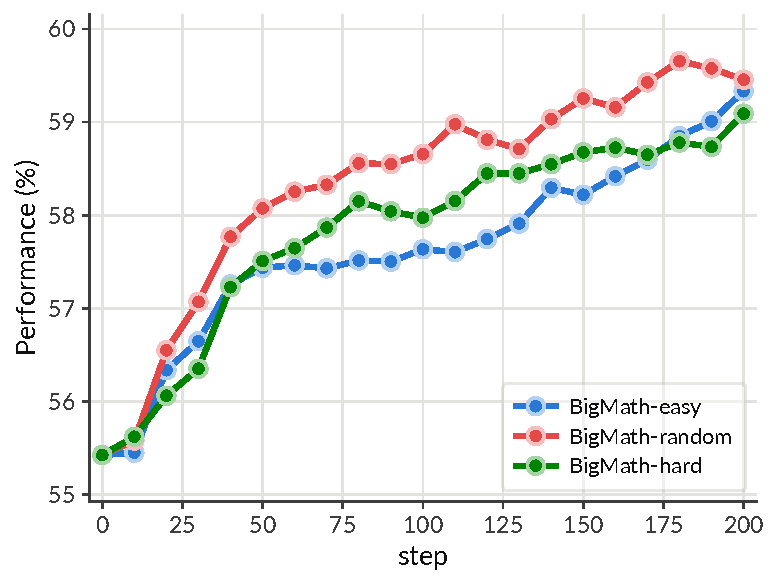
\includegraphics[width=\linewidth]{latex/figures/findings_1/teacher_pass_rate/32b_to_8b_math_teacher_pass_rate_mainmath6_avg.pdf}
        \caption{Qwen3-32B $\rightarrow$  Qwen3-8B-SFT}
        \label{fig:teacher_pass_32b_to_8b}
    \end{subfigure}
    \hfill
    \begin{subfigure}[b]{0.32\linewidth}
        \centering
        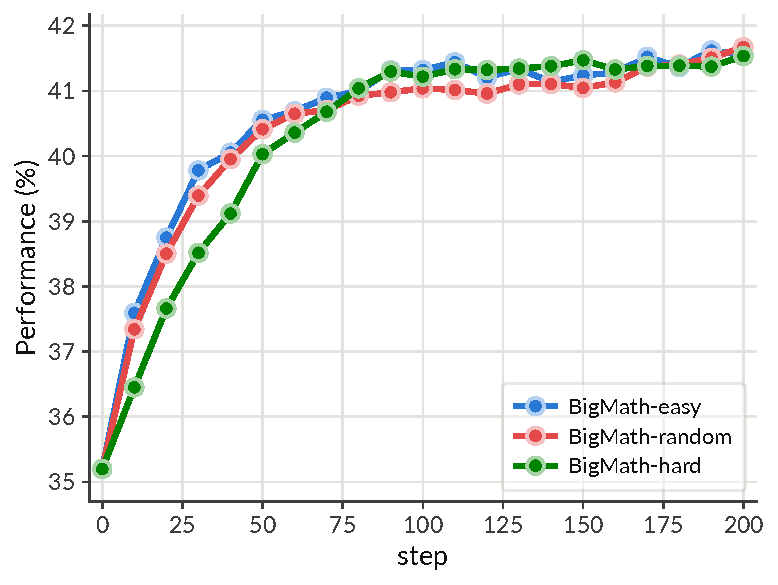
\includegraphics[width=\linewidth]{latex/figures/findings_1/teacher_pass_rate/7b_to_1d5b_math_teacher_pass_rate_mainmath6_avg.pdf}
        \caption{Polaris-7B $\rightarrow$ DS-distill-1.5B}
        \label{fig:teacher_pass_7b_to_1d5b}
    \end{subfigure}
    \hfill
    \begin{subfigure}[b]{0.32\linewidth}
        \centering
        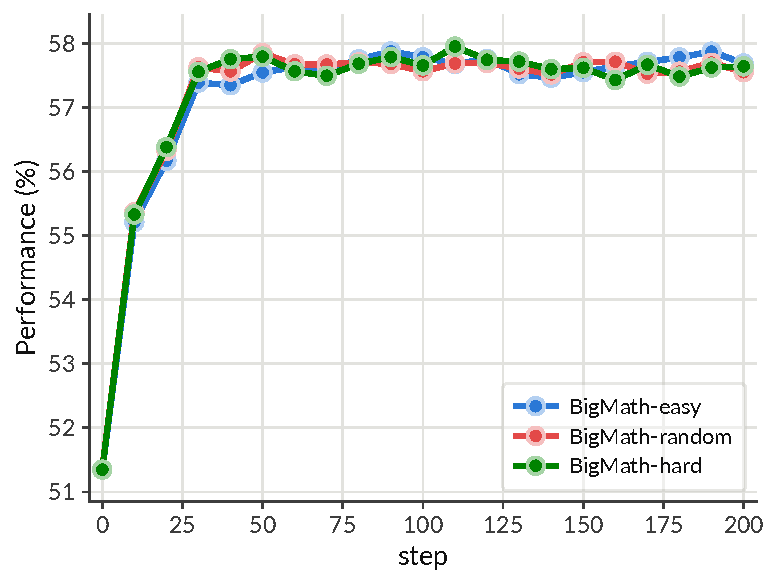
\includegraphics[width=\linewidth]{latex/figures/findings_1/teacher_pass_rate/7b_to_7b_math_teacher_pass_rate_mainmath6_avg.pdf}
        \caption{Polaris-7B $\rightarrow$ DS-distill-7B}
        \label{fig:teacher_pass_7b_to_7b}
    \end{subfigure}

    \caption{领域内数学准确率（六项英文基准的平均值）对训练问题的难度不敏感，该难度由教师模型的通过率衡量。每个图表比较了三个BigMath子集：\textbf{简单}（通过率 $=1$ ，教师解决全部四个回溯），\textbf{困难}（通过率 $=0$ ，教师一个也未解决），以及 \textbf{随机}（从整个数据集中随机采样）。这三个子集在所有教师-学生组合下最终准确率均收敛至几乎相同水平。}
    \label{fig:teacher_pass_rate_combined}
\end{figure*}
\begin{table*}[htbp]
\centering
\caption{OPD 在六项数学基准上的泛化性能，采用学生端动态采样。仅丢弃学生已解决的问题（通过率 $\in[0,1)$）时，平均性能最佳。绿色/红色标记表示相对于无动态采样基准的每项基准性能提升/下降。}
\label{tab:pass-rate-eval}
\resizebox{\textwidth}{!}{%
\begin{tabular}{c|cccccc|c}
\toprule
\textbf{Filtering Strategy} & \textbf{AMC2023} & \textbf{MATH500} & \textbf{AIME2025} & \textbf{AIME2026} & \textbf{BeyondAIME} & \textbf{OlymMATH-Hard} & \textbf{Average} \\
\midrule
\midrule
\multicolumn{8}{c}{\textbf{\textit{Teacher: Polaris-7B, Student: DS-distill-1.5B}}} \\
\midrule
\textbf{w/o dynamic sampling} & $80.4\%$ & $89.5\%$ & $30.2\%$ & $30.1\%$ & $13.6\%$ & $4.7\%$ & $41.4\%$ \\
\midrule
\textbf{pass-rate} $\mathbf{= 0}$        & \cellcolor{red!25}$78.8\%$ & \cellcolor{green!25}$90.1\%$ & \cellcolor{green!25}$30.5\%$ & \cellcolor{red!25}$30.0\%$ & \cellcolor{green!25}$14.7\%$ & \cellcolor{red!25}$4.4\%$ & $41.4\%$ \\
\textbf{pass-rate} $\mathbf{= 1}$        & \cellcolor{red!25}$79.9\%$ & \cellcolor{green!25}$89.7\%$ & \cellcolor{green!25}$30.9\%$ & \cellcolor{red!25}$28.9\%$ & \cellcolor{green!25}$14.7\%$ & \cellcolor{red!25}$4.0\%$ & $41.4\%$ \\
\textbf{pass-rate} $\mathbf{\in [0, 1)}$ & \cellcolor{green!25}$80.9\%$ & \cellcolor{green!25}$89.8\%$ & \cellcolor{green!25}$31.2\%$ & \cellcolor{green!25}$31.1\%$ & \cellcolor{green!25}$13.7\%$ & \cellcolor{green!25}$5.4\%$ & $\mathbf{42.0}\%${\footnotesize \textcolor{green!60!black}{(\textbf{+0.6 pp})}} \\
\midrule
\midrule
\multicolumn{8}{c}{\textbf{\textit{Teacher: Light-R1-14B, Student: DS-distill-7B}}} \\
\midrule
\textbf{w.o. dynamic sampling} & $91.7\%$ & $95.0\%$ & $42.8\%$ & $49.7\%$ & $26.5\%$ & $8.7\%$ & $52.4\%$ \\
\midrule
\textbf{pass-rate} $\mathbf{= 0}$        & \cellcolor{green!25}$92.1\%$ & \cellcolor{red!25}$94.3\%$ & \cellcolor{red!25}$40.2\%$ & \cellcolor{green!25}$50.3\%$ & \cellcolor{green!25}$28.2\%$ & \cellcolor{red!25}$7.8\%$ & $52.1\%${\footnotesize \textcolor{red!60!black}{(\textbf{-0.3 pp})}} \\
\textbf{pass-rate} $\mathbf{= 1}$        & \cellcolor{green!25}$92.3\%$ & \cellcolor{red!25}$94.5\%$ & \cellcolor{red!25}$42.2\%$ & \cellcolor{red!25}$48.7\%$ & \cellcolor{green!25}$28.0\%$ & \cellcolor{red!25}$8.0\%$ & $52.2\%${\footnotesize \textcolor{red!60!black}{(\textbf{-0.2 pp})}} \\
\textbf{pass-rate} $\mathbf{\in [0, 1)}$ & \cellcolor{green!25}$92.1\%$ & \cellcolor{green!25}$95.4\%$ & \cellcolor{green!25}$43.2\%$ & \cellcolor{green!25}$50.6\%$ & \cellcolor{green!25}$28.0\%$ & \cellcolor{red!25}$7.5\%$ & $\mathbf{52.8}\%${\footnotesize \textcolor{green!60!black}{(\textbf{+0.4 pp})}} \\
\bottomrule
\end{tabular}%
}
\end{table*}

\paragraph{学生通过率。}
我们在 BigMath 的随机子集上测试了两组模型：Polaris-7B\,$\rightarrow$ \,DS-distill-1.5B 和 Light-R1-14B\,$\rightarrow$ \,DS-distill-7B。  
对每个问题，我们采样四个学生响应，并将三种策略与无过滤基准（no-filtering baseline）进行比较：仅保留完全未解出的问题（通过率 $=0$ ）、仅保留完全解出的问题（通过率 $=1$ ），或仅丢弃完全解出的问题（通过率 $\in[0,1)$ ）。如表~\ref{tab:pass-rate-eval} 所示，限制于任一极端情形均无益处；而 \emph{\textbf{动态丢弃学生已能完全解出的问题，则为两组模型均带来微小但稳定的提升}}。该结果符合直觉：一旦学生能够稳定地解出某问题，教师便不应继续在该问题上对其推理过程进行重新对齐。综上，OPD 在领域内的泛化能力在很大程度上不受训练问题难度的影响。
\begin{insightbox}
\textbf{要点：}
动态丢弃学生已能完全解出的问题（即通过率 = 0）可带来微小但稳定的改进，表明教师不应持续对已掌握推理能力的学生进行重新对齐。
\end{insightbox}
\subsection{跨语言与推理范围的泛化}
\label{subsec:lang_horizon}

\begin{figure*}[t]
    \centering

    \begin{subfigure}[b]{0.99\linewidth}
        \centering
        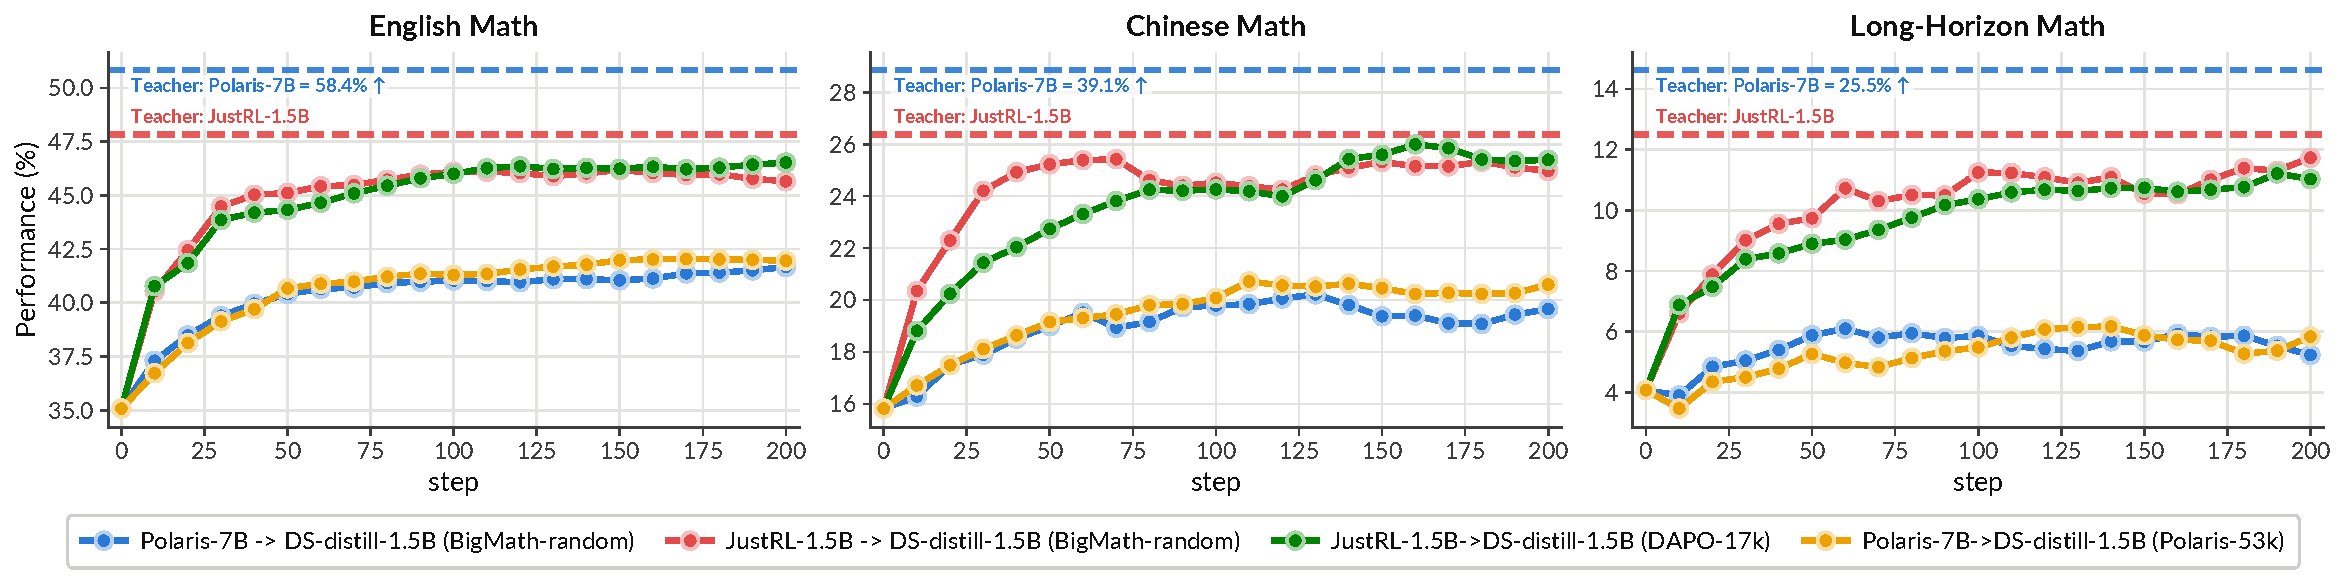
\includegraphics[width=\linewidth]{latex/figures/findings_1/1d5b_same_different_source_comparison_math_math_panel.pdf}
        \caption{DS-蒸馏-1.5B}
        \label{fig:1d5b_cross_language_horizon}
    \end{subfigure}

    \begin{subfigure}[b]{0.99\linewidth}
        \centering
        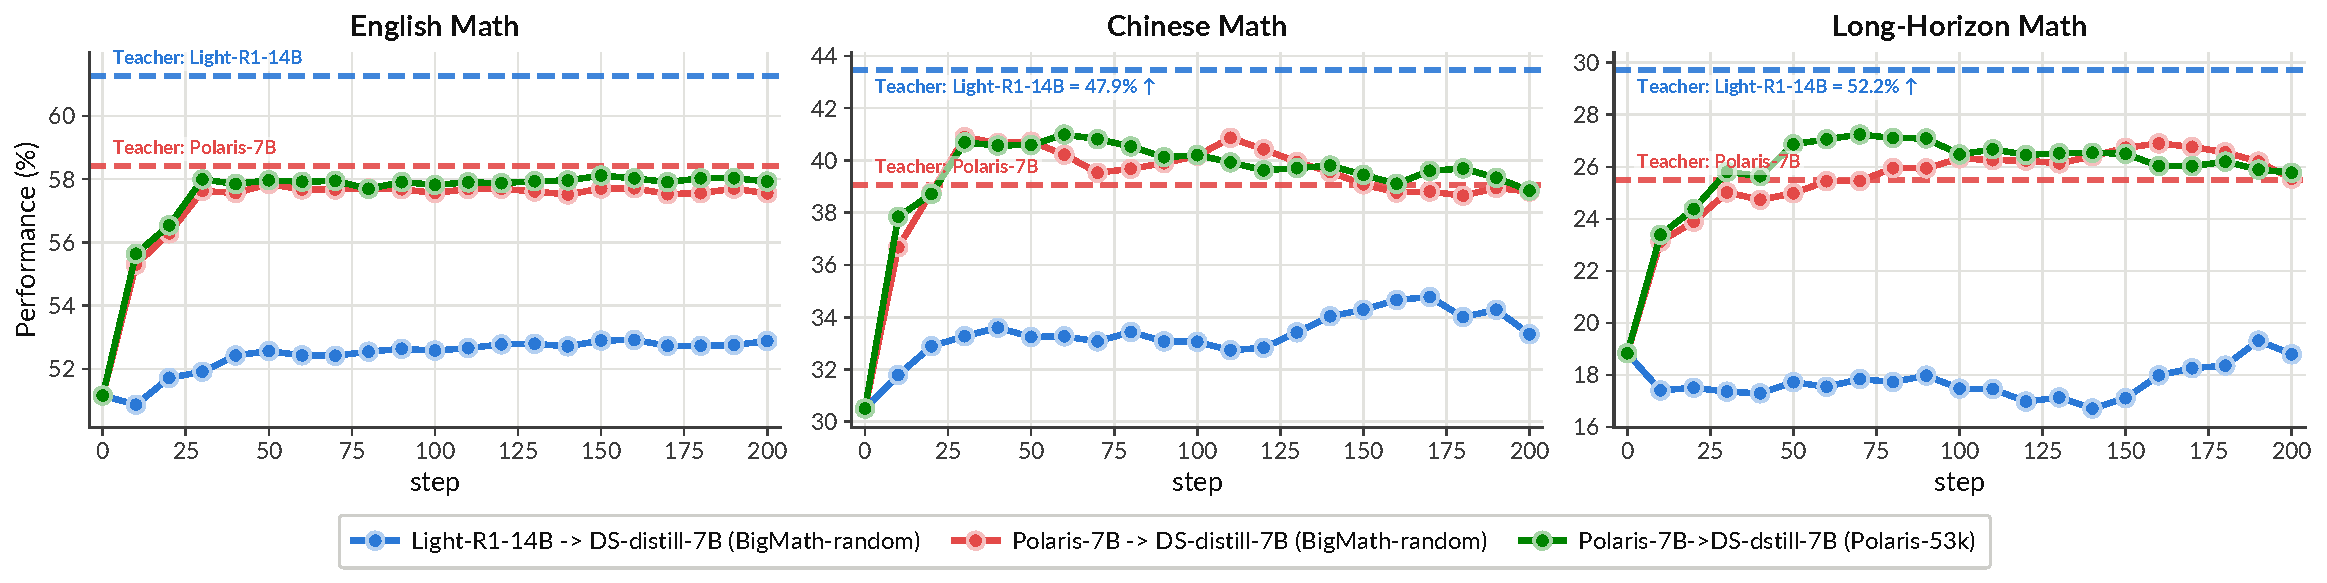
\includegraphics[width=\linewidth]{latex/figures/findings_1/7b_same_different_source_comparison_math_math_panel.pdf}
        \caption{DS-蒸馏-7B}
        \label{fig:7b_cross_language_horizon}
    \end{subfigure}

    \caption{OPD仅在英文数学题上训练，但能泛化到中文和长时程数学基准测试，然而收益的大小和稳定性取决于模型来源。每个图表中，同一学生配对了同源和跨源的教师；虚线标记了教师的准确率。}
    \label{fig:cross_language_and_horizon_same_different_origin}
\end{figure*}

我们探讨所获得的推理能力是否能泛化到两种偏移分布上：(1) 训练数据为英文数学题，而评估数据为中文数学题；(2) 训练问题原本是原子性的且短时域的，而评估问题为长时域~\citep{dziri2023faith, shojaee2025the,lu2025r}，由\emph{多个数学问题组合而成}；这考察了系统性泛化能力。我们评估两名学生，DS-distill-1.5B/7B，每名学生分别配对一个同源教师和一个跨源教师，所有模型均在BigMath-random上进行训练。图~\ref{fig:cross_language_and_horizon_same_different_origin}显示，\emph{\textbf{OPD不仅提升了分布内英文数学题的表现，还提升了中文和长时域分布的表现}}。仅在英文数据上训练即可提升中文数学题的准确率，说明所获得的能力并不依赖于训练问题的表面语言；在长时域基准上也出现了性能提升，这些题目需要长时域推理以及在子问题间传递中间答案，而这种结构在训练数据中并不存在。然而，同源教师与跨源教师之间的性能提升幅度存在显著差异，我们将在下文进一步分析。

\paragraph{模型原点的作用。}
\label{subsec:origin_indomain}
对于每个学生，我们在图~\ref{fig:cross_language_and_horizon_same_different_origin} 中比较了在同源教师与跨源教师下的 OPD 泛化表现（例如，对于 DS-distill-1.5B，JustRL-1.5B 是同源教师，而 Polaris-7B 是跨源教师）。有两个观察尤为突出。  
首先，\emph{\textbf{更强的教师并不意味着更强的学生：同源教师远比跨源教师更有效}}。例如，在 7B 面板中，跨源的 Light-R1-14B 在独立评估中的准确率明显高于同源的 Polaris-7B（虚线），但其生成的学生模型却弱得多，并且在长推理链数学任务上，跨源学生模型相较于初始模型几乎没有任何显著提升。其次，\emph{\textbf{同源 OPD 能使学生模型始终接近教师的准确率，这一点不仅体现在分布内英文评估中，也适用于语言和推理长度的分布外情况}}。一个合理的解释是，原点可作为教师策略与学生之间兼容性的一个指示器，因此 \emph{\textbf{同源配对能够整体对齐，并将这种对齐能力跨分布传递}}。  
此外，实证结果还表明，使用教师的 RL 训练提示（例如，Polaris-7B 使用 Polaris-53k，JustRL-1.5B 使用 DAPO-17k）在 OPD 性能上并未带来显著差异。

\begin{insightbox}
\textbf{要点：}
OPD 也能在领域内分布变化的情况下工作，但主要是在同一原点情景下：仅在英语、短时程数学上训练的学生，在拥有同一原点教师时，能够在中文和长时程数学上接近教师的水平，而拥有跨原点教师（即使其表现优于同一原点教师）时，提升幅度较小。
\end{insightbox}



\begin{figure*}[t]
    \centering
    \captionsetup[subfigure]{font=footnotesize}
    \begin{subfigure}[b]{0.32\linewidth}
        \centering
        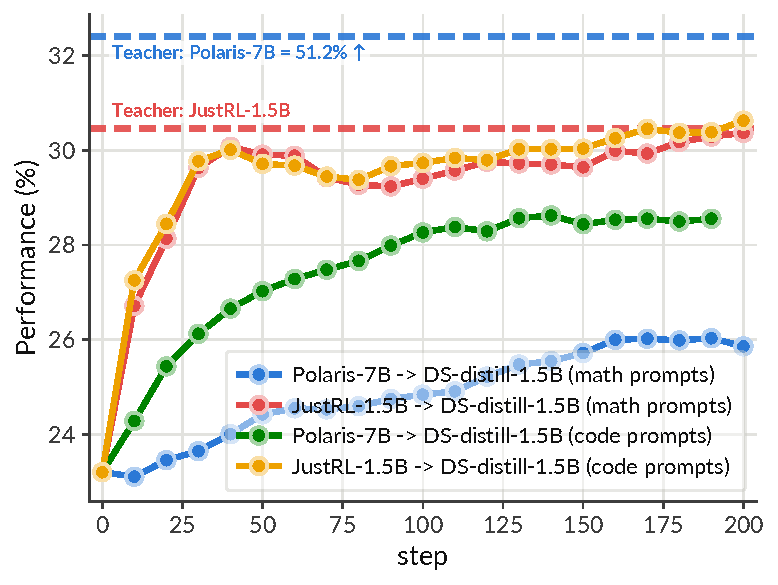
\includegraphics[width=\linewidth]{latex/figures/findings_2/1d5b_cross_domain_generalization_code_avg.pdf}
        \caption{LiveCodeBench (DS-distill-1.5B)}
        \label{fig:math_to_code_1d5b}
    \end{subfigure}
    \hfill
    \begin{subfigure}[b]{0.32\linewidth}
        \centering
        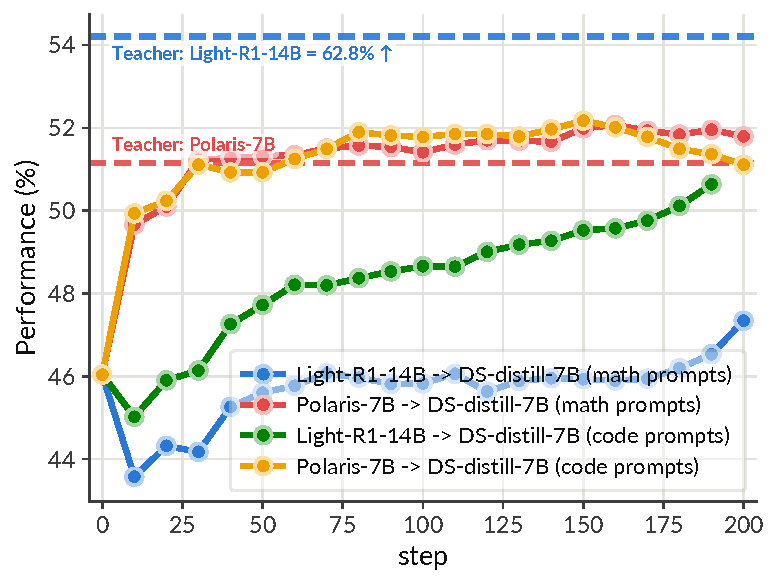
\includegraphics[width=\linewidth]{latex/figures/findings_2/7b_cross_domain_generalization_code_avg.pdf}
        \caption{LiveCodeBench（DS-distill-7B）}
        \label{fig:math_to_code_7b}
    \end{subfigure}
    \hfill
    \begin{subfigure}[b]{0.32\linewidth}
        \centering
        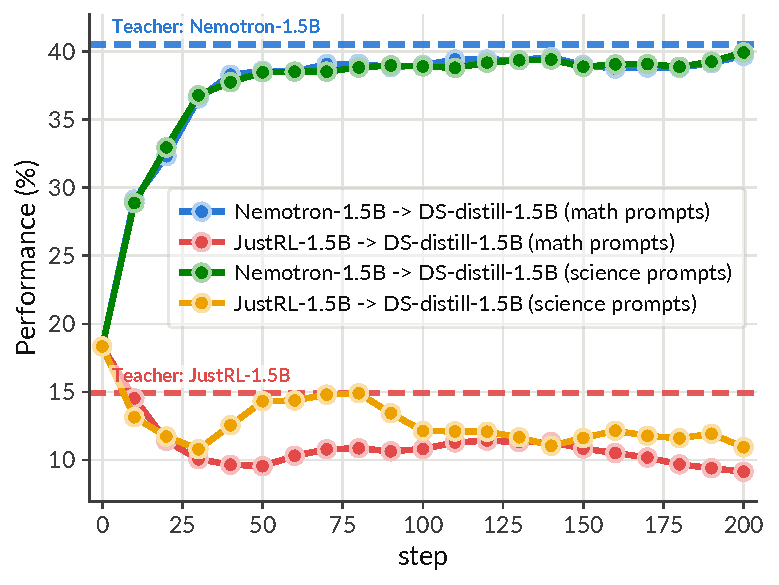
\includegraphics[width=\linewidth]{latex/figures/findings_2/1d5b_cross_domain_generalization_science_gpqa_avg.pdf}
        \caption{GPQA-钻石版（DS-精炼-1.5B）}
        \label{fig:math_to_science_1d5b}
    \end{subfigure}

     \begin{subfigure}[b]{0.99\linewidth}
        \centering
        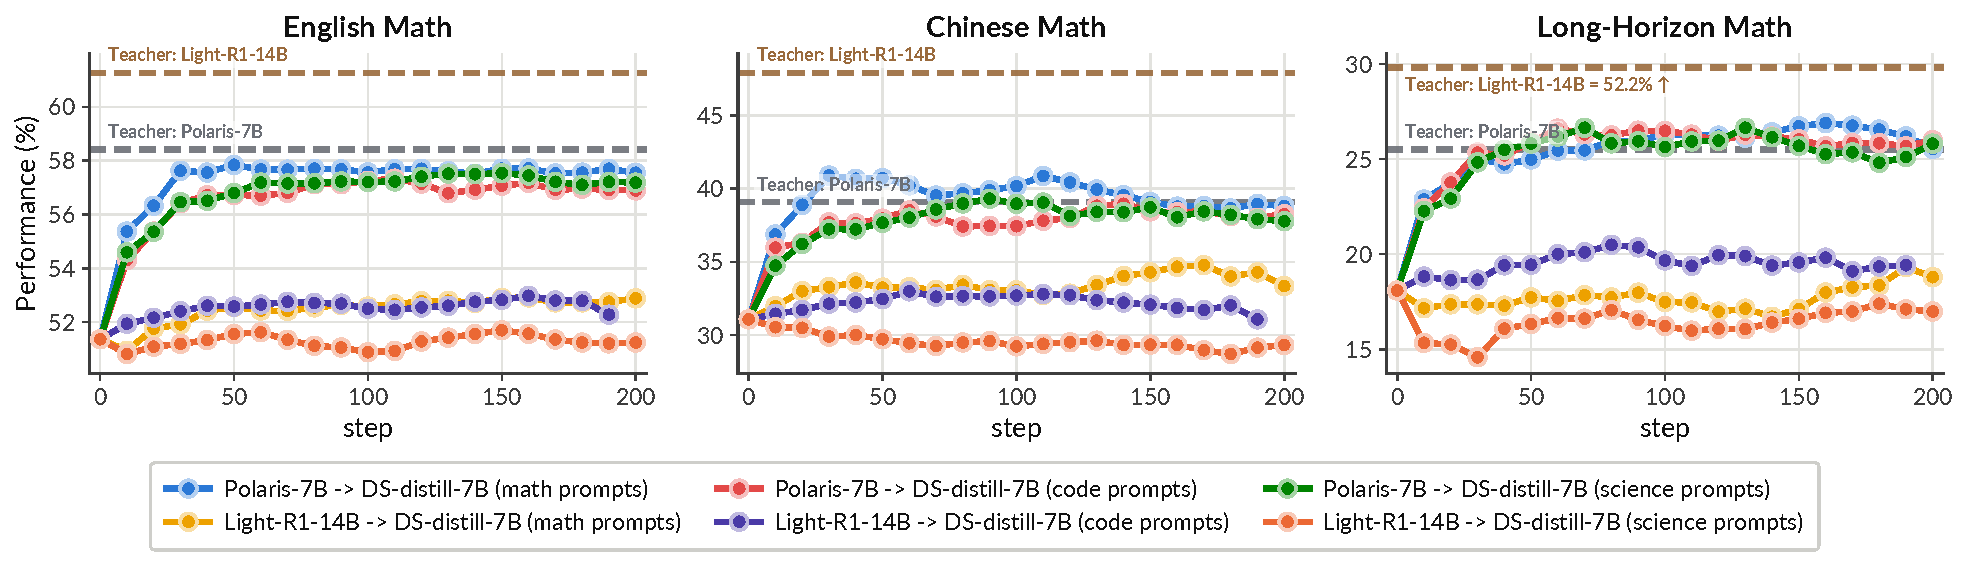
\includegraphics[width=\linewidth]{latex/figures/findings_2/7b_cross_domain_generalization_others_to_math_panel.pdf}
        \caption{在非数学领域进行训练，在数学领域进行评估（DS-distill-7B）}
        \label{fig:generalize_to_math_7b_panel}
    \end{subfigure}

    \caption{跨领域泛化在单教师OPD中的表现。对于同源OPD，基于数学提示进行训练时，学生在科学和代码任务上的表现也趋近于教师的表现，反之亦然。而对于跨源OPD，跨领域泛化性能显著下降：在(a)和(b)（LiveCodeBench评估结果）中，\textcolor{green!80!black}{绿色曲线}（基于代码提示训练）始终明显高于\textcolor{blue}{蓝色曲线}（基于数学提示训练）。虚线标记了教师单独训练的准确率。}
    \label{fig:cross_domain_generalization_math_to_others}
\end{figure*}
\section{跨领域泛化及其对多任务开放域问答的影响}
\label{sec:cross_domain}
我们现在转向跨领域泛化，即在某一领域的提示上执行OPD，并在其他领域上进行评估，以及其对MOPD的启示。本节提出两个相互关联的发现。首先，在同源OPD设置下，仅在某一领域的提示上进行训练，也能使学生在其他领域的表现接近教师的表现。相比之下，跨源设置中，跨领域泛化与域内泛化之间存在明显差距。因此，同源教师的影响并不局限于其训练提示所在的领域；在MOPD中将提示路由至不同领域的专家教师，并不能隔离它们的影响；调整教师混合比例会使得学生在各领域专家之间来回摆动，产生一种\emph{跷跷板效应}。
\subsection{OPD的跨领域泛化}
在跨领域泛化方面，我们研究了两个学生模型：DS-distill-1.5B 和 DS-distill-7B，并将每个学生模型分别与同源和跨源教师模型配对；例如，对于 DS-distill-1.5B，JustRL-1.5B 和 Nemotron-1.5B 是同源教师模型，而 Polaris-7B 是跨源教师模型。我们以两个方向运行 OPD：一是基于数学（教师模型强化学习后训练的领域）的提示进行训练，然后在代码和科学等其他领域进行评估；二是基于其他领域的提示（代码、科学和 IF）进行训练，然后在数学领域进行评估。
\paragraph{数学 $\rightarrow$  其他领域迁移。}
我们首先在数学提示上训练学生，然后在代码和科学任务上进行评估。如图~\ref{fig:math_to_code_1d5b} 和~\ref{fig:math_to_code_7b} 所示，尽管在OPD过程中未使用代码提示，但1.5B和7B的学生在LiveCodeBench上的得分均明显提升。科学任务上也出现了类似现象：如图~\ref{fig:math_to_science_1d5b} 所示，在数学和科学提示训练下，Nemotron-1.5B与JustRL-1.5B的表现对比显示了相同趋势。对于以科学为导向的Nemotron教师，经过数学或科学提示训练的学生最终达到相近的GPQA-Diamond得分水平，均显著高于初始学生得分。然而，由于以数学为导向的JustRL教师的科学推理能力弱于学生，因此无论采用数学还是科学提示进行训练，都会导致学生表现下降，最终使其GPQA得分低于初始水平。

\paragraph{其他领域 $\rightarrow$  数学迁移。}
如图~\ref{fig:generalize_to_math_7b_panel} 所示，使用代码或科学提示进行训练的学生在数学任务上表现提升（接近教师水平），且性能提升不仅限于英语，还扩展到中文和长时程数学基准。

这些结果表明，即使使用非主要领域的提示，教师的专长能力（即数学推理）也能传递给学生（见图~\ref{fig:if_to_math_cross_domain_generalization} 中的 IF$\rightarrow$ 数学迁移情况）。

综上所述，这些结果表明 \textbf{\emph{OPD 可以将能力从其训练提示的语义领域之外进行迁移：来自数学推理的监督信号能够引导学生在代码/科学推理能力上向教师靠拢，反之亦然}}。

\begin{insightbox}
\textbf{要点：}
OPD 可以在两个方向上将同一来源教师的能力从其训练提示的领域拓展出去：在数学提示上进行训练可提升学生在代码和科学方面的能力，而在代码、科学或指令遵循提示上进行训练则能反向提升数学能力，且提升效果延伸至中文和长序列数学问题。
\end{insightbox}

\paragraph{在OPD中，模型的泛化能力因模型来源而异。}
模型原点，首次出现在第~\ref{subsec:origin_indomain} 节，再次在跨领域情景中清晰显现。在图~\ref{fig:math_to_code_1d5b} 和~\ref{fig:math_to_code_7b} 中，同源教师在 LiveCodeBench 上对 \textcolor{yellow!85!black}{代码提示} 训练和 \textcolor{red}{数学提示} 训练均展现出一致的训练曲线：两者均 \textbf{趋近于} 教师的表现，因此在同源 OPD 情景下，训练领域差距基本消除，学生即使仅从数学轨迹中也能吸收教师的代码能力。

而跨源 OPD 的表现则截然不同：直接在目标领域进行训练仍为最优，我们观察到在领域内泛化（使用 \textcolor{green!80!black}{代码提示} 训练）与跨领域泛化（使用 \textcolor{blue}{数学提示} 训练）之间存在 \textbf{明显差距}。

我们将这一差异归因于教师与学生之间的分布差距。对于一个 \textit{\underline{同源教师}}，其输出分布相较于学生仅经过微调~\citep{yue2025does}，\textbf{\emph{OPD 在策略层面而非仅在训练领域上使学生与教师对齐}}。然而，对于一个 \emph{\underline{跨源教师}}，更大的分布差距使得这种对齐更加困难，\textbf{\textit{OPD 主要将学生策略拉向教师策略，且仅限于训练提示所覆盖的分布范围}}，导致跨领域泛化能力弱于领域内泛化。

\begin{insightbox}
\textbf{要点：}
跨领域迁移的范围受到模型原点的影响。同源教师模型（其分布与学生模型接近）即使在提示仅来自单一领域的情况下，也能使学生模型在跨领域上达到接近教师模型的水平，有效缩小训练领域间的差距。而异源教师模型面对更大的分布差异，在训练分布上的表现有所提升，但其跨领域泛化能力明显低于其领域内泛化能力。 
\end{insightbox}
\begin{figure*}[t]
    \centering
    \begin{subfigure}[b]{0.99\linewidth}
        \centering
        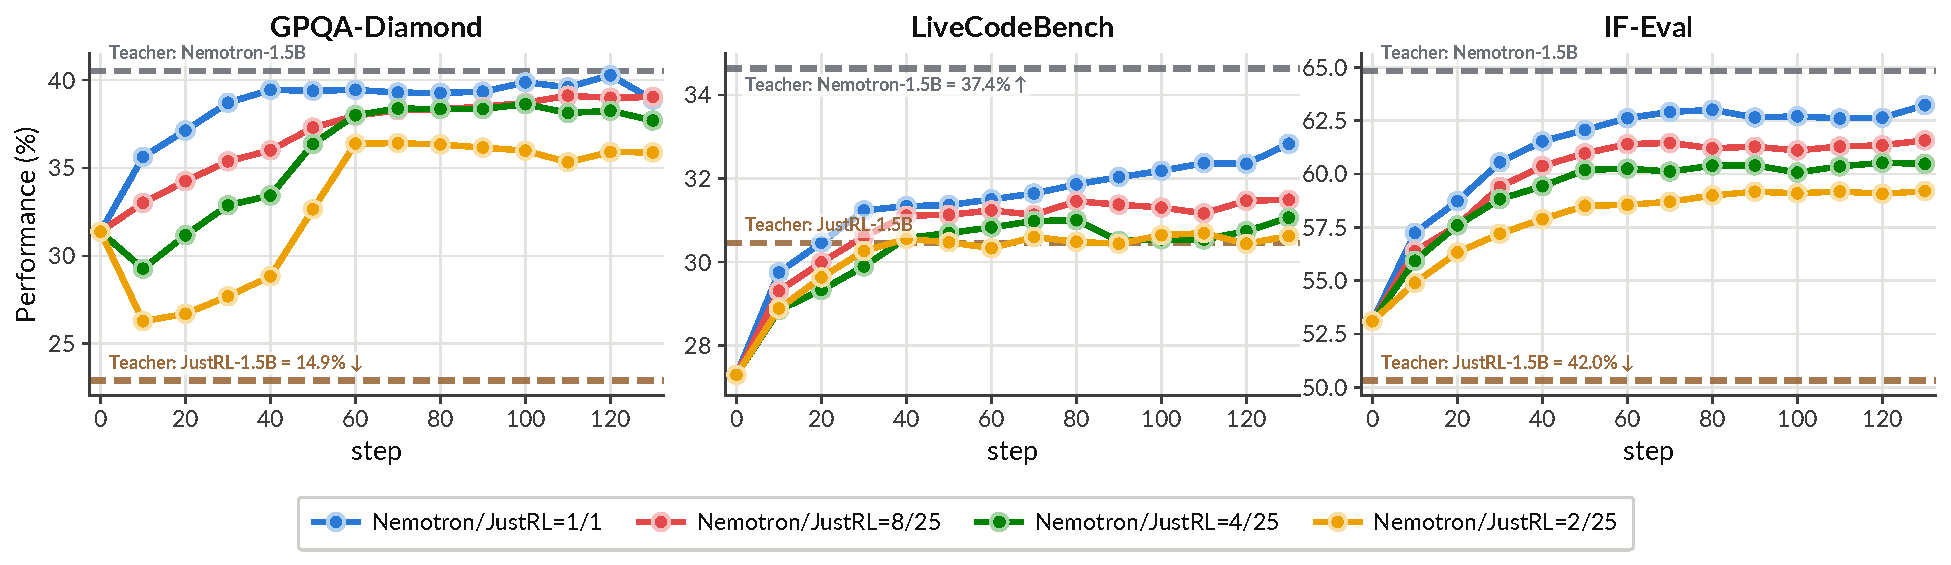
\includegraphics[width=\linewidth]{latex/figures/findings_3/mopd_nemo10step_panel.pdf}
        \caption{情景1. 数学老师：JustRL-1.5B；科学/如果老师：Nemotron-1.5B；学生：Dev-1.5B。}
        \label{fig:mopd_nemo10step}
    \end{subfigure}

    \begin{subfigure}[b]{0.99\linewidth}
        \centering
        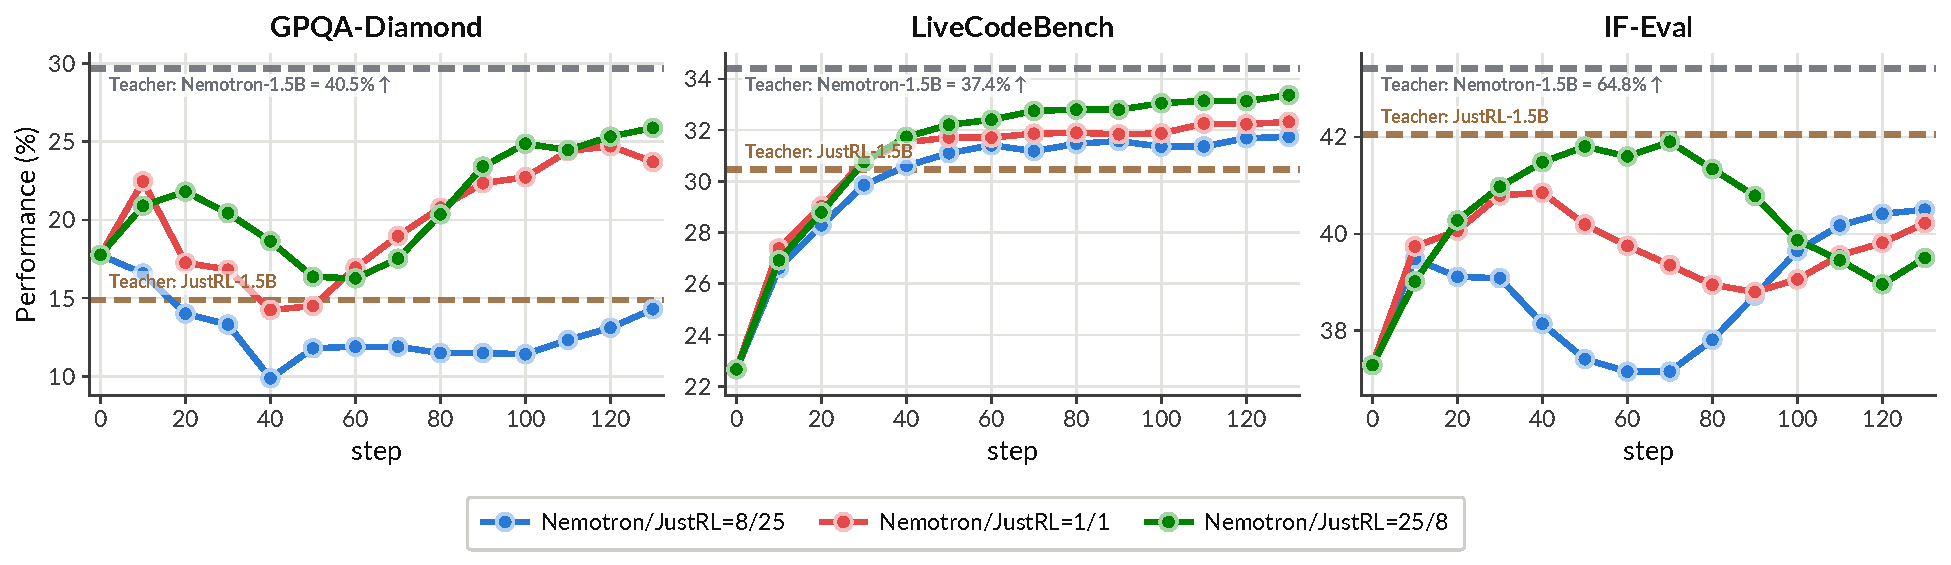
\includegraphics[width=\linewidth]{latex/figures/findings_3/mopd_reverse_teacher_panel.pdf}
        \caption{情景2. 数学老师：Nemotron-1.5B；科学/信息学老师：JustRL-1.5B；学生：DS-distill-1.5B。}
        \label{fig:mopd_reverse_teacher}
    \end{subfigure}

    \caption{\textbf{\emph{MOPD跷跷板效应}}。改变不同教师分配提示的混合比例，会显著影响OPD学生在不同领域的能力。例如，在子图(a)中，随着JustRL-1.5B（数学教师）数据比例的增加，学生的GPQA-Diamond（科学推理）、LiveCodeBench（代码推理）和IF-Eval（指令遵循）性能逐渐下降。}
    \label{fig:mopd_seesaw_effect}
\end{figure*}
\subsection{MOPD中的跨领域干扰}
\label{subsec:mopd}

\begin{table}[t]
\centering
\caption{不同JustRL-1.5B/Nemotron-1.5B混合比例（J/N）下的MOPD数学准确率。}
\label{tab:mopd-step200}
\resizebox{0.6\columnwidth}{!}{%
\begin{tabular}{c|cc|c}
\toprule
\textbf{Config} & \textbf{BeyondAIME} & \textbf{OlymMATH} & \textbf{Average} \\
\midrule
\midrule
DS-distill-1.5B & $9.6\%$ & $14.2\%$ & $11.9\%${\footnotesize \textcolor{black!60!black}{(\textbf{student})}} \\
\midrule
\midrule
\multicolumn{4}{c}{\textbf{\textit{Math Teacher: JustRL-1.5B, Science/IF Teacher: Nemotron-1.5B}}} \\
\midrule
$\mathbf{\text{J}/\text{N}=25/2}$ & $19.4\%$ & $33.3\%$ & $26.4\%${\footnotesize \textcolor{green!60!black}{(\textbf{+0.1 pp})}} \\
$\mathbf{\text{J}/\text{N}=25/8}$ & $19.6\%$ & $34.5\%$ & $27.1\%${\footnotesize \textcolor{green!60!black}{(\textbf{+0.8 pp})}} \\
$\mathbf{\text{J}/\text{N}=1/1}$ & $20.2\%$ & $32.4\%$ & $26.3\%${\footnotesize \textcolor{black!60!black}{(\textbf{baseline})}} \\
$\mathbf{\text{J}/\text{N}=8/25}$ & $19.7\%$ & $32.5\%$ & $26.1\%${\footnotesize \textcolor{red!60!black}{(\textbf{-0.2 pp})}} \\
$\mathbf{\text{J}/\text{N}=2/25}$ & $19.2\%$ & $31.0\%$ & $25.1\%${\footnotesize \textcolor{red!60!black}{(\textbf{-1.2 pp})}} \\
\midrule
\midrule
\multicolumn{4}{c}{\textbf{\textit{Math Teacher: Nemotron-1.5B, Science/IF Teacher: JustRL-1.5B}}} \\
\midrule
$\mathbf{\text{J}/\text{N}=25/8}$ & $17.4\%$ & $28.0\%$ & $22.7\%${\footnotesize \textcolor{green!60!black}{(\textbf{+0.7 pp})}} \\
$\mathbf{\text{J}/\text{N}=1/1}$ & $17.3\%$ & $26.6\%$ & $22.0\%${\footnotesize \textcolor{black!60!black}{(\textbf{baseline})}} \\
$\mathbf{\text{J}/\text{N}=8/25}$  & $17.1\%$ & $26.2\%$ & $21.7\%${\footnotesize \textcolor{red!60!black}{(\textbf{-0.3 pp})}} \\
\bottomrule
\end{tabular}%
}
\end{table}

\begin{figure*}[t]
    \centering
    \captionsetup[subfigure]{font=scriptsize}
    \begin{subfigure}[b]{0.32\linewidth}
        \centering
        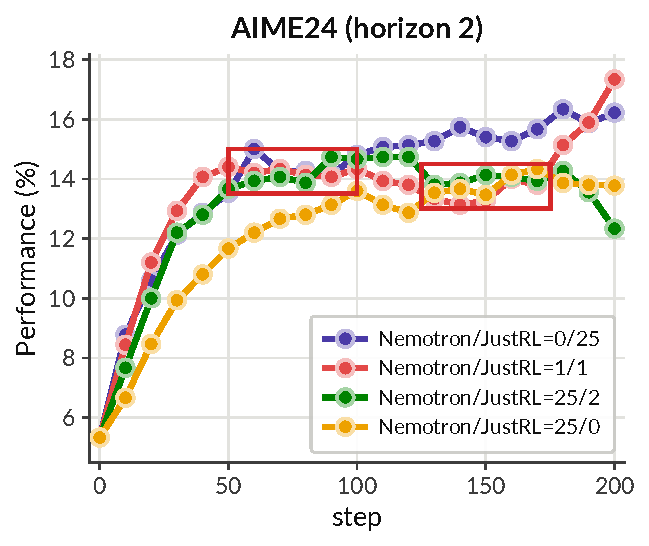
\includegraphics[width=\linewidth]{latex/figures/findings_3/mopd_forward_teacher_aime24_horizon2.pdf}
        \caption{JustRL-Math，Nemotron-Science/IF}
        \label{fig:switch_mopd}
    \end{subfigure}
    \hfill
    \begin{subfigure}[b]{0.32\linewidth}
        \centering
        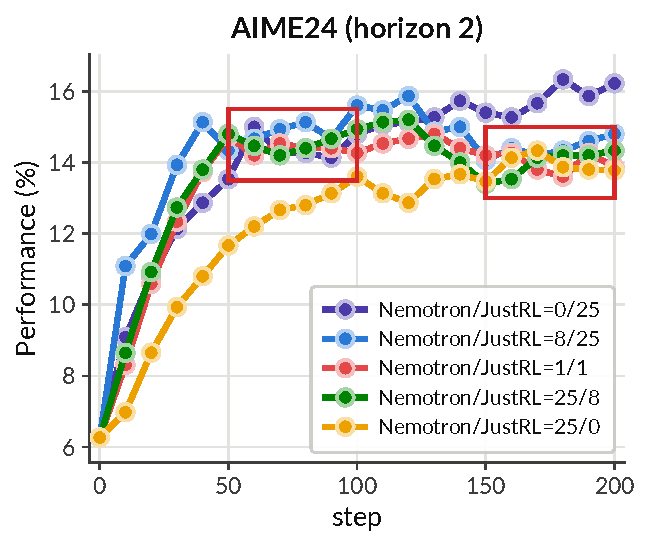
\includegraphics[width=\linewidth]{latex/figures/findings_3/mopd_reverse_teacher_aime24_horizon2.pdf}
        \caption{JustRL-Science/IF，Nemotron-Math}
        \label{fig:switch_mopd_reverse_teacher}
    \end{subfigure}
    \hfill
    \begin{subfigure}[b]{0.32\linewidth}
        \centering
        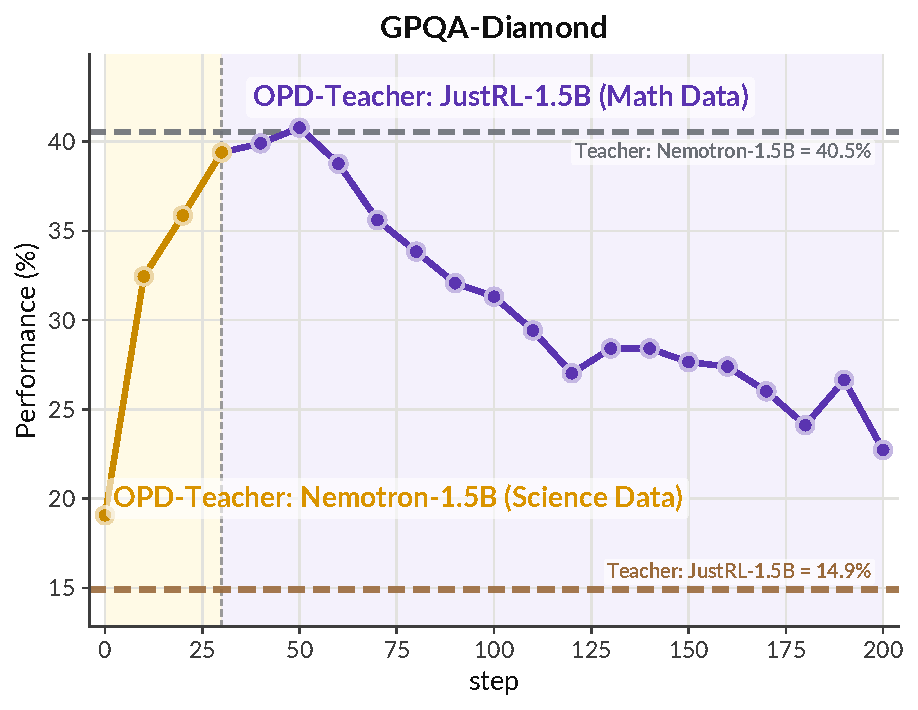
\includegraphics[width=\linewidth]{latex/figures/findings_3/mopd_teacher_switch_gpqa.pdf}
        \caption{级联OPD，GPQA-钻石}
        \label{fig:cascaded_opd}
    \end{subfigure}
    \caption{在MOPD训练过程中，教师之间的拉锯战可以被观察到。(a,b) \textcolor{red}{用红色框标出} 的部分显示，在两种情景下，MOPD学生的性能首先\textbf{\emph{跟踪}} \textcolor{violet}{仅使用JustRL的训练曲线}，随后逐渐向 \textcolor{yellow!85!black}{仅使用Nemotron的训练曲线} 偏移。(c) 在级联式OPD（先一个教师再另一个教师）中，受科学提示引导的Nemotron-1.5B指导时，GPQA性能 \textcolor{yellow!85!black}{急剧上升}，随后在数学提示引导的后续JustRL-1.5B作用下 \textcolor{violet}{回落}，从而在时间维度上解耦了多教师的影响。}
    \label{fig:additional_result_mopd}
\end{figure*}

单教师跨领域泛化观察对多教师开放领域推理（MOPD）具有关键但容易被忽视的含义：由于一个教师的影响范围远超其OPD训练提示所覆盖的领域，因此\textbf{\emph{将每个提示路由到特定领域的教师，并不能将其影响限制在分配的领域内}}。这为MOPD提出了一个实际问题：分配给不同领域的教师是否\emph{\textbf{争夺相同的能力}}，因为每个教师的跨领域影响可能与其他教师在其指定领域内的监督产生重叠和冲突。我们通过两个学生进行测试，Dev-1.5B\footnote{请参阅附录~\ref{sec:appendix_model_lineage} 以获取详细说明} 以及 DS-distill-1.5B 和两位具有互补特点的教师模型：JustRL-1.5B（在数学方面更强）和 Nemotron-1.5B（在科学和IF方面强得多，但在数学方面较弱）。在情景~1中，JustRL-1.5B 作为数学教师，Nemotron-1.5B 作为科学/IF教师。为了隔离路由提示领域的影响，并进一步探究此消彼长效应，情景~2 交换了它们的角色，使用 Nemotron-1.5B 作为数学教师，JustRL-1.5B 作为科学/IF教师，并追踪学生在各领域的表现变化。

\paragraph{教师混合比例引发跷跷板效应。}
当我们改变分配给两位教师的提示比例，同时保持其总量不变时，学生在每个基准上的表现会趋向于获得更大份额的教师，而非由教师所负责的领域决定。  
在情景~1（图~\ref{fig:mopd_nemo10step}）中，随着 JustRL（数学教师）所占份额增加（Nemotron/JustRL 从 $1/1$ 变为 $2/25$），学生的 GPQA-Diamond、LiveCodeBench 和 IFEval 得分均下降，趋近于 JustRL 较低的得分；\textbf{\emph{在 GPQA-Diamond 上，数学教师 JustRL 的拉力足够强，以至于准确率甚至在训练初期就下降了 $\sim5\%$ }}，因为 JustRL 在该指标上的得分低于学生 Dev-1.5B。在情景~2（图~\ref{fig:mopd_reverse_teacher}）中，当 Nemotron 被指定为数学教师时，同样的三个基准得分随 Nemotron 份额增加而上升，向 Nemotron 在这些基准上更高的得分靠拢。  
数学领域的结果（表~\ref{tab:mopd-step200}）给出了相反的情况：适当提高 JustRL 的份额（因其数学表现优于 Nemotron）能提升数学得分，无论其被分配到哪个领域。

最终，性能的转变不仅仅由教师指定的领域决定：\textbf{\emph{均匀增加教师的占比会将多领域能力拉向该教师的基准水平，形成一种依赖混合比例的跷跷板效应，使得针对特定领域的提示路由无法有效限制教师的影响}}。


\paragraph{训练期间可以观察到教师之间的一场拔河较量。}
最后，教师之间的平衡在训练过程中发生变化。在 AIME24-Horizon-2 的两种情景下（图~\ref{fig:switch_mopd} 和~\ref{fig:switch_mopd_reverse_teacher}），MOPD 学生最初跟随更强数学能力的 JustRL-only 曲线，随后逐渐偏离并趋向于更低的 Nemotron-only 水平，因此学生并未立即稳定在某个固定的混合结果上，而是随着训练的进行在两个教师之间不断被拉扯。

在图~\ref{fig:switch_mopd} 中，当 JustRL 作为数学教师时，我们可以观察到，最终红色曲线（Nemotron/JustRL 混合比例 $1/1$）重新被拉回至 JustRL-only 曲线，而黄色曲线（Nemotron/JustRL 混合比例 $25/2$，分配给 JustRL 的提示更少）则完全被拉向 Nemotron-only 曲线。

此外，我们还开展了一项级联 OPD 实验（图~\ref{fig:cascaded_opd}），以在时间维度上解耦多教师 OPD 训练的影响：首先使用科学能力更强的 Nemotron-1.5B 教师和科学提示进行训练，使 GPQA 提升至其水平；在切换为 JustRL-1.5B 教师和数学提示后，GPQA 又回落至原始水平。


\paragraph{跷跷板效应为分析MOPD提供了一个心理模型。}
跷跷板效应为分析MOPD~\citep{chen2026counteraction}中的抵消作用提供了一个有用的视角：当学生在某一领域表现不佳时，原因未必在于被分配至该领域的教师，因为另一名教师可通过其自身的跨领域迁移拉动相同的能力。这表明，在诊断MOPD时，应考察全部教师集合，而非仅关注所涉领域的领域专家；同时也表明，一名领域专家在其目标领域之外所具备的能力，与其在MOPD中的行为相关，而不仅限于其在所分配领域上的表现。因此，传统的提示路由范式~\citep{ma2026mopd,coreteam2026mimov2flashtechnicalreport,huang2026kat,xu2026deepseek}并不能保证不同领域专家的能力彼此隔离。

\begin{insightbox}
\textbf{要点：}
由于教师的影响不限于其OPD提示所在的领域，因此在多教师OPD（MOPD）中将提示路由给领域专家也无法将其完全隔离。随着混合比例的变化，学生在每个基准上的得分会趋向于占比更大的教师，且趋向于该教师自身的水平，而非其被分配到的领域水平。  
因此，结合专家会产生一种与混合比例相关的\emph{跷跷板}效应，而非专家技能的简单叠加。这一现象为诊断MOPD提供了有益视角：某一领域表现不佳，可能源于其他教师的跨领域影响，因此领域专家的非本领域行为同样重要。
\end{insightbox}

\section{关于同源/跨源OPD实验的更多讨论}

\begin{figure*}[t]
    \centering
    \begin{subfigure}[b]{0.48\linewidth}
        \centering
        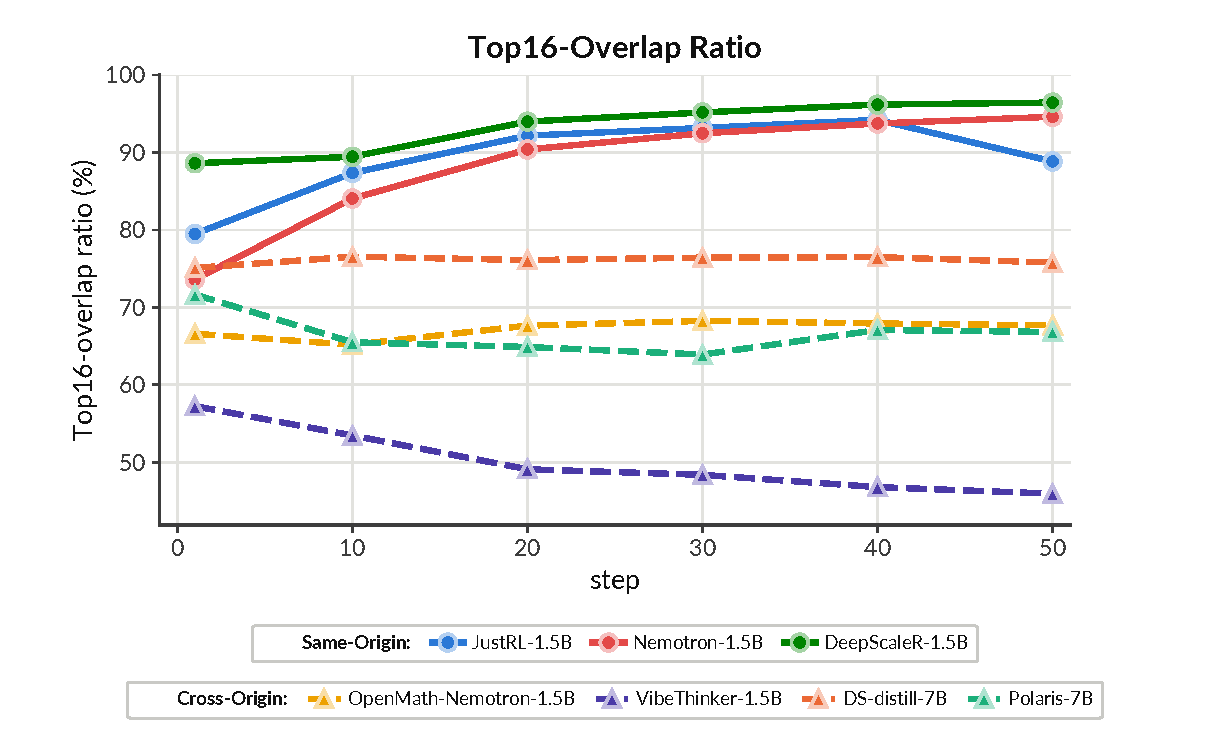
\includegraphics[width=\linewidth]{latex/figures/discussion/to_dpsk1d5b_top16_overlap.pdf}
        \caption{DS-distill-1.5B OPD 实验}
    \end{subfigure}
    \begin{subfigure}[b]{0.48\linewidth}
        \centering
        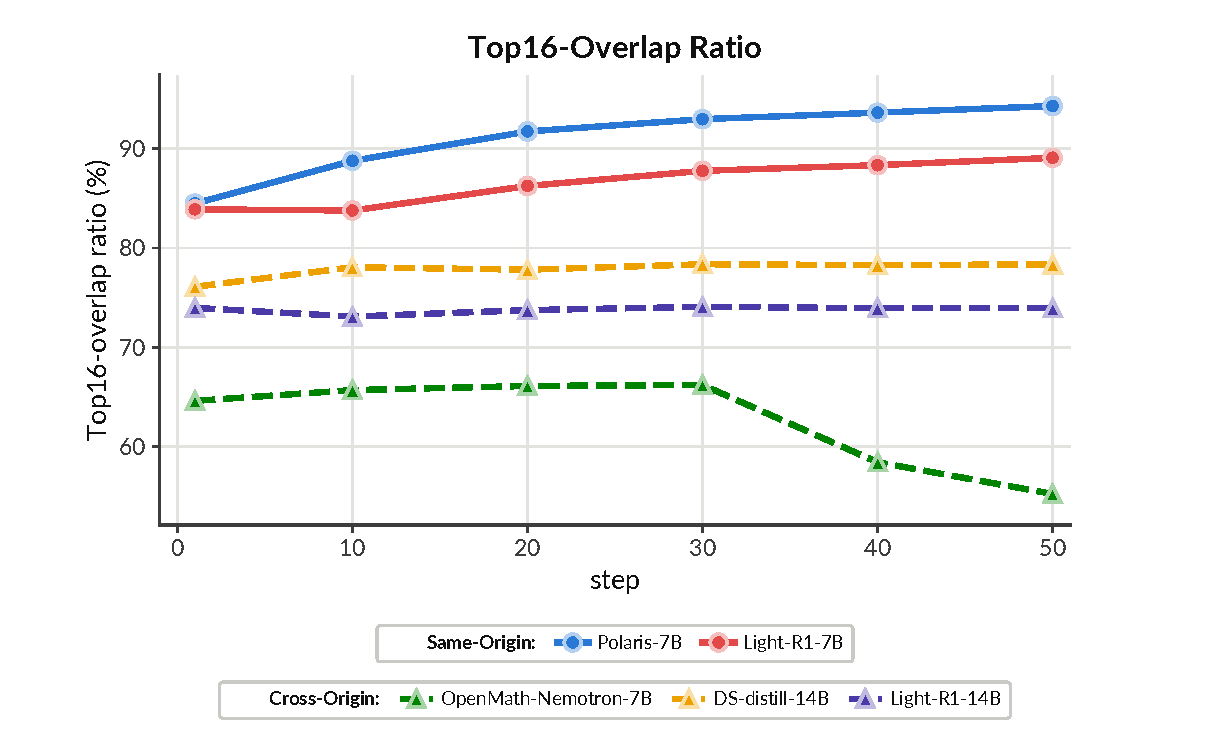
\includegraphics[width=\linewidth]{latex/figures/discussion/to_dpsk7b_top16_overlap.pdf}
        \caption{DS-distill-7B OPD 实验}
    \end{subfigure}

    \caption{不同OPD实验中教师模型与学生模型的Top-K（K=16）重叠比率。图(a)和图(b)中的学生模型分别为DS-distill-1.5B和DS-distill-7B。实线表示使用同原点教师模型的OPD实验；虚线表示使用不同原点教师模型的OPD实验。}
    \label{fig:top16_overlap_ratio}
\end{figure*}

\begin{figure}[htbp]
    \centering
    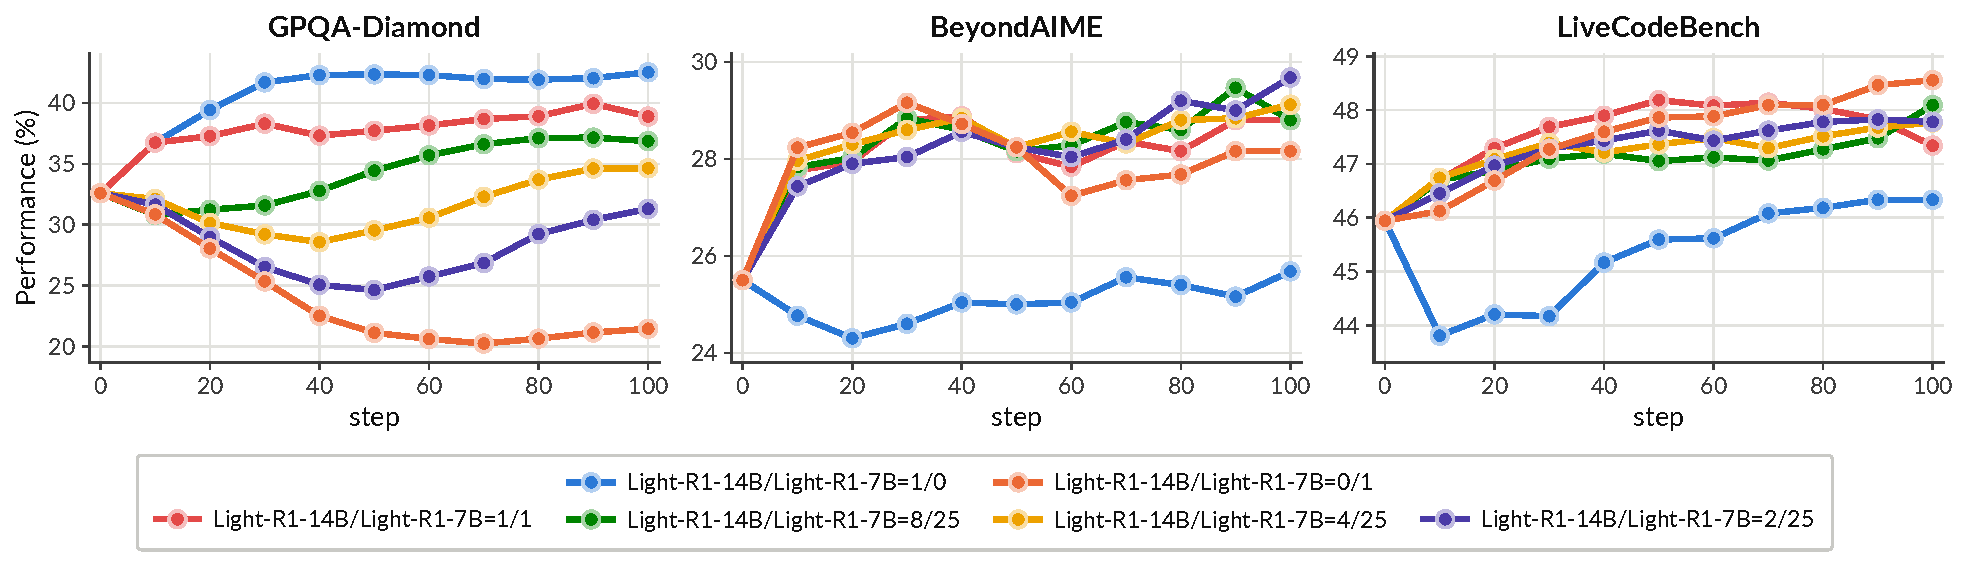
\includegraphics[width=0.99\linewidth]{latex/figures/discussion/mopd_light_14b_7b_panel.pdf}
    \caption{DS-distill-7B（学生）的MOPD实验结果，以及Light-R1-7B（数学教师）和Light-R1-14B（科学/推理教师）的实验结果。图例表示不同MOPD实验中专家数据混合比例（Light-R1-14B/Light-R1-7B $\in\{1/0, 1/1, 8/25, 4/25, 2/25, 0/1\}$ ）。}
    \label{fig:mopd_7b}
\end{figure}

在整篇论文中，模型原点始终是区分广泛泛化与狭窄拟合的最关键因子。我们最后通过两项分析更直接地探讨了原因：一是OPD如何在训练过程中重塑学生模型的策略，二是在MOPD中同源教师与异源教师竞争时，这种影响的具体表现。

\paragraph{同源OPD将学生的策略作为一个整体进行对齐。}
为了探究 OPD 如何在训练损失之外改变学生策略，我们测量了在训练过程中教师与学生下一个 token 分布之间的 top-$K$ ($K{=}16$ ) 重叠比率~\citep{li2026rethinking}（见图~\ref{fig:top16_overlap_ratio}）。
1.5B 和 7B 的学生均表现出两种一致的模式。
首先，相同原点的教师对应的重叠比率明显高于跨原点的情况，这证实了在任何 OPD 之前，共享原点已使学生策略更接近教师策略。
其次，更具启示性的是，相同原点的重叠比率在训练过程中显著上升，而跨原点的重叠比率则保持平稳甚至下降。
由于两种情景都最小化相同的教师-学生 KL 目标，这一对比表明：相同原点的 OPD 逐步实现学生对教师策略的全面对齐，而跨原点的 OPD 仅在训练分布上减少散度，却未能促使两策略达成更广泛的共识。
这为“相同原点可泛化，跨原点仅拟合”提供了机制解释：广泛迁移源于整体策略对齐，而这种对齐在教师与学生共享原点时更容易实现。

\paragraph{同源教师在MOPD中产生的引力更强。}
当将同源教师与跨源教师结合时，同样的不对称性再次显现。我们在 DS-distill-7B 上重复了 MOPD 实验，使用同源的 Light-R1-7B 作为数学教师，以及跨源的 Light-R1-14B 作为科学/IF 教师（图~\ref{fig:mopd_7b}）。在 GPQA-Diamond 上，即使在 $1{:}1$ 平衡混合比例下，科学教师获得相等份额，学生的科学准确率仍迅速向数学教师 Light-R1-7B 靠拢。结合上述对齐分析可知，在 MOPD 中，同源教师对学生的影响力强于跨源教师，因此教师之间的天平不仅受混合比例影响，还受到每个教师与学生原点接近程度的影响。

\begin{insightbox}
\textbf{要点：}
同源OPD在训练过程中提高了教师-学生模型的前$K$ 重叠度，而跨源OPD则没有，因此广泛泛化来自于整体对齐学生策略，而非仅仅降低在训练分布上的KL散度。因此，同源教师对学生的牵引力强于跨源教师，从而在起源和混合比例两个方面都倾斜了MOPD的天平。
\end{insightbox}
\section{结论}
我们通过受控地改变训练和评估分布，从领域内偏移到跨领域迁移，研究OPD的泛化能力。OPD对训练问题的难度变化基本不敏感，能够将其教师的能力迁移到训练提示所属领域的外部，但主要限于同源配对。由于路由机制无法将教师的影响限制在其分配的领域内，因此在MOPD中整合领域专家会导致它们能力之间的此消彼长，而非专家技能的独立组合，这一现象为诊断MOPD提供了有益视角。
\section*{局限性}

我们的实验聚焦于推理导向的模型，涵盖数学、代码、科学和指令遵循等领域的任务。所观察到的泛化模式可能无法直接推广至多模态、工具使用或交互式智能体的情景。
将分析扩展到此类任务有助于判断当监督信号依赖外部观测或动作时，OPD是否表现出类似的跨领域行为。
此外，我们的MOPD实验考虑了两个能力互补的教师，并采用基于固定领域的提示路由策略。
这种受控设置使得单个教师的跨领域效应更容易分析，但实际系统可能涉及更大且更异构的专家池。
它们也可能采用自适应路由机制和非均匀的教师采样策略。对专家池大小和路由策略的更广泛研究将有助于更全面地理解MOPD中的泛化行为。

\section*{道德考虑}
本研究探讨了公开可用语言模型在数学、代码、科学及指令遵循基准上的能力迁移。我们的结果表明，OPD能够将教师模型的行为迁移至路由训练提示所属领域之外的领域。尽管这实现了广泛的能力迁移，但也可能将教师模型中的不良行为或偏见传播到训练过程中未明确监控的领域。

特别是，在MOPD中进行提示路由时，不应将其视为严格的能力或安全边界。因此，使用OPD或MOPD训练的模型应全面评估其在所有领域中的安全性与可靠性，而不仅限于每个教师所对应的特定领域。



\bibliography{ref}

\appendix
\section{相关工作}
\label{appendix:related_work}

\subsection{大规模后训练中的OPD}



传统的知识蒸馏通常在教师生成的响应上训练学生模型，导致训练过程中观察到的序列与学生在推理时生成的序列之间存在不匹配。GKD通过获取教师对学生生成序列的反馈来减少这种不匹配~\cite{agarwal2024policy}。MiniLLM进一步将语言模型蒸馏形式化为反向KL最优化，并开发了一种同策略策略梯度估计量\cite{gu2024minillm}。最近，思维机器实验室提出了OPD，作为一种实用的后训练范式，结合了学生端的探索与稠密的token级教师监督~\cite{lu2025onpolicydistillation}。


OPD及其多教师变体随后成为大规模大模型后训练的重要组成部分。近期的技术报告利用它们来整合独立训练的领域专家，并将多种能力融合到单一模型中~\cite{
coreteam2026mimov2flashtechnicalreport,
xu2026deepseek,
yang2026nemotron,
huang2026kat,
team2026mach}。这些研究为OPD的实际有效性与可扩展性提供了有力证据。然而，它们主要评估最终集成模型的表现，而未系统地分离在训练和评估分布受控变化下，提炼出的能力是否具备泛化性~\citep{li2026rolereasoningpatternsgeneralization,ren2026rethinkinggeneralizationreasoningsft,chu2025sft,garcia2025exploringllmscapturerepresent}。

\subsection{理解OPD机制}


最近的研究探讨了OPD取得成功所需的条件。
\citet{li2026rethinking} 将兼容的教师-学生思维模式和真正新颖的教师能力识别为有效蒸馏的两个重要因素。


其他研究则关注OPD的最优化病态问题。
\citet{fu2026revisiting} 分析了采样 token 最优化中的偏差与方差，识别出学生生成前缀的不可靠指导以及分词器不匹配为主要失效模式。  
一项互补研究将 OPD 描述为一种探索机制，并强调学生-教师不匹配和长度利用是两种核心病理~\cite{wang2026demystifying}。


多种方法通过修改其展开或最优化过程来提升OPD性能。  
早停OPD将监督限制在较早的响应位置，从而降低教师指导受学生前缀漂移的影响 \cite{ziheng2026less}。  
非对称OPD对正向量和非正向量优势采用不同的最优化处理方式，以平衡利用与模仿 \cite{jia2026asymmetric}。  
尽管这些研究解释并缓解了局部训练失败问题，我们关注的是一个互补性问题：OPD是否能在难度、语言、推理范围、任务领域以及模型原点之间实现迁移。

\subsection{OPD中的数据选择}


数据选择在大语言模型推理的强化学习中得到了广泛研究~\cite{yu2026dapo,kong2026rethinking,li2025learnalign}。  
越来越多的工作通过选择或重新加权其监督信号来改进OPD。  
SCOPE将正确的学生轨迹与错误的学生轨迹分离，强调教师对错误回放轨迹的纠正置信度以及学生对正确轨迹的不确定性~\cite{zheng2026scope}。  
FiRe-OPD首先过滤不可靠的轨迹，然后对保留轨迹中的信息性token进行软重加权~\cite{li2026filter}。  
BRTS采样多个教师轨迹，并根据教师的正确性以及与当前学生的对齐程度来选择监督信号~\cite{zhang2026policy}。  
Uni-OPD通过双视角策略，联合考虑学生侧的探索和教师侧的监督可靠性~\cite{hou2026uni}。


这些方法在不同粒度上选择监督信号，但并未直接决定是否应过滤教师未解决的查询，或保留学生已掌握的查询。我们通过受控的教师端过滤和学生端动态采样，将这两个因子分离，并进一步比较它们在不同模型原点情景下的影响。

\subsection{MOPD中的能力交互}


多教师同策略蒸馏（MOPD）通过将学生生成的轨迹路由至对应的教师，实现对单个学生的逐 token 监督~\cite{ma2026mopd}。在集成前独立训练领域专家，MOPD 降低了异构强化学习目标之间的直接耦合，并提供了一种可扩展的能力集成方法。


然而，来自多个教师的监督可能并不相互兼容。CaMOPD识别出由冲突的教师梯度引起的恢复—保持对抗效应，以及由于对具有不同修正需求的样本进行均匀组合而导致的弱信号平坦化现象\cite{chen2026counteraction}。它通过解耦最优化和基于教师-学生差距的样本选择来解决这些问题。


我们的工作从互补的跨领域泛化视角研究能力交互。我们不仅将每个教师视为仅传递其名义上的专长技能，还考察其更广泛的能力特征如何传递到主要领域和非主要领域。

\section{实验情景}
\label{sec:appendix_exp_setting}

\subsection{数据集}
\label{sec:appendix_datasets}

\subsubsection{训练数据集}
\label{sec:appendix_training_datasets}

\paragraph{数学推理}

我们使用 Big-Math-RL-Verified~\cite{albalak2025big} 作为主要的数学训练语料库。  
在绝对难度对比中，可用的 GSM8K~\cite{cobbe2021traininggsm8k} 和 DeepMath-103K-Hardest~\cite{he2026deepmathk} 语料库各自包含约 8K 个查询。  
因此，我们从 Big-Math-RL-Verified 中采样一个匹配的 8K 查询子集，以确保对比结果不受唯一训练查询数量的影响。

\paragraph{代码推理。}

我们使用 DeepCoder-Preview-Dataset~\cite{deepcoder2025} 进行代码领域 OPD。该数据集包含约 24K 个编程竞赛题目，每个题目都配有可执行的测试用例。其训练集包括从 2023 年 5 月 1 日到 2024 年 7 月 31 日期间提交的 LiveCodeBench~\cite{jain2025livecodebench} 题目，以及来自 TACO~\cite{li2023taco} 和 PrimeIntellect 的 SYNTHETIC-1~\cite{2025synthetic1} 的已验证题目。

\paragraph{科学推理。}

在单教师跨领域实验中，我们使用TextbookReasoning~\cite{fan2025megascience}作为科学领域的训练语料库。我们移除了所有标注为数学或计算机科学的样本，以减少与数学和代码领域的直接重叠。在MOPD实验中，我们遵循Nemotron-Research-Reasoning-Qwen-1.5B~\cite{liu2026prorl}训练所用的数据领域。科学数据来自SCP-116K~\cite{lu2025scp}，在过滤掉所有归类为数学的样本后获得。


\paragraph{指令执行。}

MOPD 中使用的指令遵循数据来自 Llama-Nemotron-后训练数据集~\cite{bercovich2025llamanemotron} 的 RL/指令遵循划分。我们将这些示例与筛选后的 SCP-116K 数据一起，构建科学/指令遵循训练池。科学和指令遵循示例各占科学/指令遵循池的 $50\%$。

\subsubsection{评估基准}
\label{sec:appendix_evaluation_datasets}

\paragraph{英语数学推理}

英语数学得分是 AMC~2023~\cite{MAA_AMC}、MATH-500~\cite{hendrycks2021measuringmath500}、AIME~2025/2026~\cite{MAA_AIME}、BeyondAIME~\cite{bytedance_seed_2025_beyondaime} 以及 OlymMATH-Hard~\cite{sun2026olymmath} 得分的平均值。

\paragraph{中国数学推理。}

中文数学得分是 OlymMATH-ZH~\cite{sun2026olymmath} 和 LiveMathBench-ZH~\cite{liu2025livemathbench} 的平均得分。

\paragraph{长期推理的数学问题。}

长期预测数学得分是 R-HORIZON~\cite{lu2025r} 中 AIME24-Horizon-2 和 AMC23-Horizon-4 的平均得分。

\paragraph{代码推理。}

我们在 2024 年 8 月 1 日至 2025 年 2 月 1 日期间发布的 LiveCodeBench v5 问题上评估代码生成能力~\cite{jain2025livecodebench}，采用 DeepCoder 所使用的评估方法。


\paragraph{科学与指令遵循。}

我们在 GPQA-Diamond~\cite{rein2023gpqa} 上评估科学推理能力，在 IFEval~\cite{zhou2023instructionfollowingevaluationlargelanguage} 上评估指令遵循能力。  
GPQA-Diamond 包含物理学、化学和生物学领域的专家级问题，而 IFEval 用于评估对可程序验证指令的遵守情况。



\subsection{模型}
\label{sec:appendix_models}

\subsubsection{模型谱系}
\label{sec:appendix_model_lineage}

我们使用模型谱系来区分同源和跨源OPD之间的差异。具体而言，当两个模型共享相同的实际初始化检查点，并且其中一个或两个模型都是从该检查点进一步进行后训练得到时，这两个模型被视为同源。

根据此定义，DeepSeek-R1-Distill-Qwen-1.5B~\cite{guo2025deepseekr1} 构成一个谱系根节点。  
JustRL-DeepSeek-1.5B~\cite{he2025justrl} 是通过对该检查点应用面向数学的强化学习后训练得到的，而  
Nemotron-Research-Reasoning-Qwen-1.5B~\cite{liu2026prorl} 则是通过从相同初始化状态进行长时间多领域强化学习获得的。  
Dev-1.5B 也从 DeepSeek-R1-Distill-Qwen-1.5B 初始化，并通过 10 步科学/IF OPD 进一步训练。  
因此，这四个模型属于同一谱系。  
DeepSeek-R1-Distill-Qwen-7B 与 Polaris-7B~\cite{Polaris2025} 构成第二个谱系，因为 Polaris-7B 是对 7B 版本的蒸馏检查点进一步后训练所得。  
同样地，DeepSeek-R1-Distill-Qwen-14B 与 Light-R1-14B~\cite{wen2025lightr1} 构成第三个谱系。  
对于 Qwen3 模型，Qwen3-4B~\cite{yang2025qwen3} 与 Polaris-4B 属于同一谱系，因为 Polaris-4B 是从 Qwen3-4B 后训练而来。  
Qwen3-8B 与 Qwen3-32B 被视为独立的谱系根节点，因为二者之间不存在彼此通过后训练获得的关系。

\begin{table*}[t]
    \centering
    \small
    \caption{
    我们实验中所用模型的后训练谱系。  
共享相同谱系根的模型被视为同源。
    }
    \label{tab:model_lineage}
    \resizebox{\linewidth}{!}{
    \begin{tabular}{llll}
        \toprule
        \textbf{Model} &
        \textbf{Lineage Root} &
        \textbf{Post-Training from the Root} &
        \textbf{Experimental Role} \\
        \midrule

        DS-R1-Distill-Qwen-1.5B
        & DS-R1-Distill-Qwen-1.5B
        & None
        & Student \\

        JustRL-DeepSeek-1.5B
        & DS-R1-Distill-Qwen-1.5B
        & Math-oriented RL
        & Teacher \\

        Nemotron-Research-Reasoning-Qwen-1.5B
        & DS-R1-Distill-Qwen-1.5B
        & Multi-domain prolonged RL
        & Teacher \\

        Dev-1.5B
        & DS-R1-Distill-Qwen-1.5B
        & 10-step science/IF OPD
        & Student \\

        \midrule

        DS-R1-Distill-Qwen-7B
        & DS-R1-Distill-Qwen-7B
        & None
        & Student \\

        Polaris-7B
        & DS-R1-Distill-Qwen-7B
        & Math-oriented RL
        & Teacher \\

        \midrule

        DS-R1-Distill-Qwen-14B
        & DS-R1-Distill-Qwen-14B
        & None
        & Student \\

        Light-R1-14B
        & DS-R1-Distill-Qwen-14B
        & Long-CoT reasoning RL
        & Teacher \\

        \midrule

        Qwen3-4B
        & Qwen3-4B
        & None
        & Student \\

        Polaris-4B
        & Qwen3-4B
        & Math-oriented RL
        & Teacher \\

        \midrule

        Qwen3-8B-SFT
        & Qwen3-8B
        & SFT on OpenThoughts3-1.2M
        & Student \\

        \midrule

        Qwen3-32B
        & Qwen3-32B
        & None
        & Teacher \\

        \bottomrule
    \end{tabular}
    }
\end{table*}

\subsection{训练配置}
\label{sec:training_config}

大多数配置在 100--200 步内收敛，因此我们将最大步数设置为 200。  
提示词批量大小为 128，每轮运行最多可使用 $200\times128=25.6$ K 个提示词实例。  
对于每个提示词，学生模型生成四个独立的同策略响应，对应于轨迹组大小为 $N=4$。  
标准的轨迹解码参数为：温度 $1.0$，top-$p$  $1.0$，以及无限制的 top-$k$ 采样，实现方式为 top-$k=-1$。

最大序列长度取决于教师-学生配置，如表~\ref{tab:max_sequence_length} 所总结。

\begin{table*}[t]
    \centering
    \caption{用于OPD推出和评估的最大序列长度。}
    \label{tab:max_sequence_length}
    \resizebox{0.8\linewidth}{!}{
    \begin{tabular}{lc}
        \toprule
        \textbf{Model Group} &
        \textbf{Maximum Length} \\
        \midrule

        Qwen3-4B, Qwen3-8B, Qwen3-32B, Polaris-4B
        & 40K \\

        DS-distill-1.5B,
        JustRL-1.5B, Nemotron-1.5B
        & 96K \\

        Light-R1-14B, DS-distill-14B
        & 64K \\

        Polaris-7B, DS-distill-7B 
        & 96K \\

        \bottomrule
    \end{tabular}
    }
\end{table*}



\subsection{评估配置}


在基准评估中，我们使用温度 $1.0$ ，top-$p$  $0.95$ ，
以及 top-$k=-1$ 。  
最大序列长度遵循
表~\ref{tab:max_sequence_length}。  
对于每个查询，我们独立采样 $K$ 个响应，并报告
$\operatorname{Avg@}K$ ，定义为

\begingroup
\begin{align*}
    \operatorname{Avg@}K
    =
    \frac{1}{|\mathcal{D}|}
    \sum_{x\in\mathcal{D}}
    \frac{1}{K}
    \sum_{k=1}^{K}
    \mathcal{V}\!\left(x,y^{(k)}\right),
    \label{eq:avg_at_k}
\end{align*}
\endgroup

其中 $y^{(k)}$  是第 $k$ 个独立采样的响应，  
$\mathcal{V}$  是特定于基准的验证器。  
与 Pass@$K$ 不同，Avg@$K$ 独立评估每个采样响应，  
并且不从 $K$ 次生成中选择最佳响应。

每个基准所使用的评估样本数量汇总于表~\ref{tab:evaluation_sampling_num} 中。

\begin{table}[t]
    \centering
    \caption{
    用于基准评估的独立采样响应数量。
    }
    \label{tab:evaluation_sampling_num}
    \resizebox{0.3\columnwidth}{!}{
    \begin{tabular}{lc}
        \toprule
        \textbf{Benchmark} & \textbf{Metric} \\
        \midrule

        AMC 2023
        & Avg@16 \\

        MATH-500
        & Avg@1 \\

        AIME 2025
        & Avg@16 \\

        AIME 2026
        & Avg@16 \\

        BeyondAIME
        & Avg@5 \\

        OlymMATH-Hard
        & Avg@5 \\

        OlymMATH-Easy
        & Avg@5 \\

        OlymMATH-ZH
        & Avg@5 \\

        R-HORIZON
        & Avg@10 \\

        LiveMathBench-ZH
        & Avg@16 \\

        GPQA-Diamond
        & Avg@4 \\

        LiveCodeBench v5
        & Avg@10 \\

        IFEval
        & Avg@4 \\

        \bottomrule
    \end{tabular}
    }
\end{table}


仅用于可视化，我们使用中心移动平均对评估曲线进行平滑处理。
令 $\{s_t\}$ 表示原始评估序列，
$\widetilde{s}_t$ 表示显示的值。
我们计算

\begingroup
\begin{align*}
    \widetilde{s}_t
    =
    \begin{cases}
        s_1,
        & t=1, \\[2pt]
        \displaystyle
        \frac{1}{3}\sum_{j=1}^{3}s_j,
        & t=2, \\[8pt]
        \displaystyle
        \frac{1}{5}\sum_{j=t-2}^{t+2}s_j,
        & t\geq 3.
    \end{cases}
\end{align*}
\endgroup

因此，第一个显示的点未进行平滑处理，第二个点对前一个、当前和后一个检查点进行平均，后续所有点均使用半径为二的五点中心移动平均。
原始训练轨迹在图中所示最终步数之外仍有延伸，因此从第三个点开始，所有显示的点均可获得完整的五点窗口，包括靠近右侧边界处的点。
中心移动平均常用于抑制局部波动，同时保留序列的主要趋势\citep{hyndman2018forecasting}。
平滑仅用于可视化，不影响任何报告的表格数值、检查点选择或统计计算。

\subsubsection{答案提取指令}
对于所有数学和科学推理基准，我们添加系统提示，并从每个模型的响应中提取最终 \texttt{\textbackslash boxed\{\}} 表达式内的答案，然后使用 Math-Verify\footnote{\url{https://github.com/huggingface/Math-Verify}} 用于解析和比较提取的答案与参考答案的库。  
对于数学任务，我们提示模型将最终答案（通常是数字和数学表达式，有时是选项）放在 \texttt{\textbackslash boxed\{\}} 内。  
\begin{insightbox}  
\textbf{数学推理任务（MATH-500, AMC23, AIME25/26, BeyondAIME, ...）：}\\  
请逐步推理，并将最终答案放入 \texttt{\textbackslash boxed\{\}} 中。  
\end{insightbox}  
对于 GPQA-Diamond，我们提示模型将最终选项（A、B、C 或 D）放入 \texttt{\textbackslash boxed\{\}}。  
\begin{insightbox}  
\textbf{科学推理任务（GPQA-Diamond）：}\\  
请逐步推理，并将最终答案（仅选项，即 A、B、C 或 D）放入 \texttt{\textbackslash boxed\{\}} 中。  
\end{insightbox}  
注意，上述两个系统提示与本文所用的所有模型保持一致。




\section{额外的实验结果}
\label{sec:appendix_add_results}
\subsection{训练数据难度的额外结果}

为了进一步检验所观察到的行为是否在仅基于单一数据集构建的难度划分之外依然成立，我们引入了两个额外的数据集，代表难度谱的两极。对于极端困难的情景，我们使用 DeepMath-103K~\cite{he2026deepmathk}，该数据集提供从 1 到 9 的难度得分，并保留得分高于 8 的查询。对于极端简单的情景，我们使用 GSM8K 训练集，该数据集包含小学数学应用题。我们在这两个数据集上重复相同的 OPD 实验，以检验当训练查询几乎总是可解或几乎从不可解时，教师端通过率是否变得更加重要。

图~\ref{fig:extreme_difficulty} 展示了实验结果。在两种难度极端情况下的实验得出了相似的结论。无论是小学水平的 GSM8K 查询还是极具挑战性的 DeepMath-103K 查询，通过 OPD 均获得了显著提升，且在所有测试配置下，它们的最终平均得分差异不足两分。因此，有效的同策略监督并不要求训练查询处于狭窄的绝对难度值域内。然而，在任一难度极端上训练的模型，通常仍落后于在更具多样性的 Big-Math-RL-Verified 混合数据集上训练的模型。这表明，尽管教师通过率或绝对查询难度本身并不能单独决定一个样本是否有效，但保持对问题难度的广泛覆盖，对于实现更广泛的泛化能力仍然有益。


\begin{figure*}[t]
    \centering
    \begin{subfigure}[b]{0.32\linewidth}
        \centering
        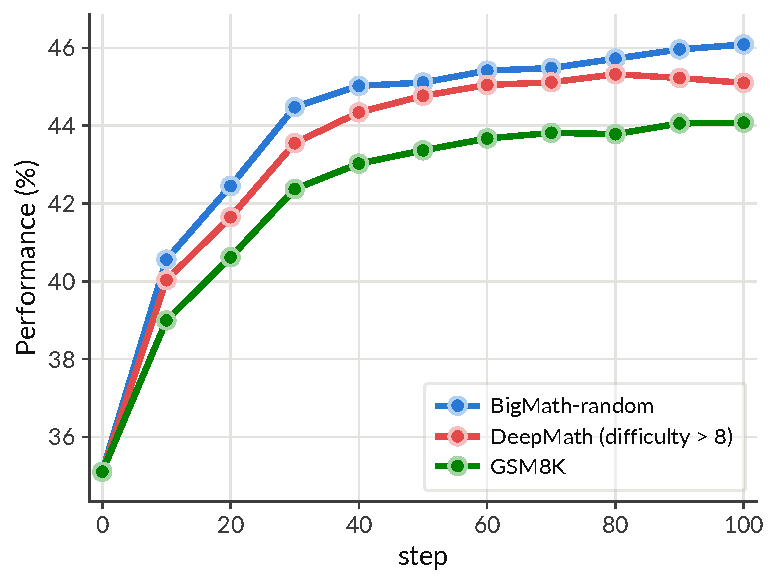
\includegraphics[width=\linewidth]{latex/figures/findings_1/teacher_pass_rate/1d5b_to_1d5b_math_teacher_difficulty_mainmath6_avg.pdf}
        \caption{JustRL-1.5B $\rightarrow$ DS-distill-1.5B}
        \label{fig:difficulty_1d5b_to_1d5b}
    \end{subfigure}
    \hfill
    \begin{subfigure}[b]{0.32\linewidth}
        \centering
        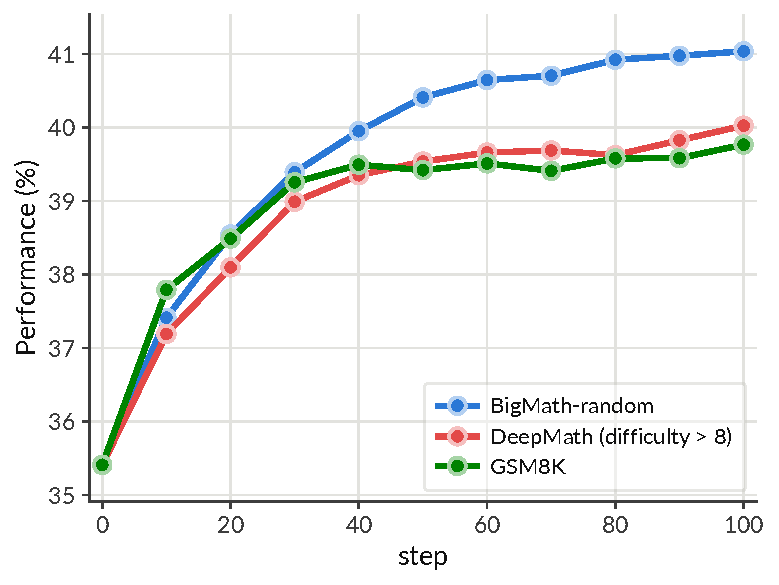
\includegraphics[width=\linewidth]{latex/figures/findings_1/teacher_pass_rate/7b_to_1d5b_math_teacher_difficulty_mainmath6_avg.pdf}
        \caption{Polaris-7B $\rightarrow$ DS-distill-1.5B}
        \label{fig:difficulty_7b_to_1d5b}
    \end{subfigure}
    \hfill
    \begin{subfigure}[b]{0.32\linewidth}
        \centering
        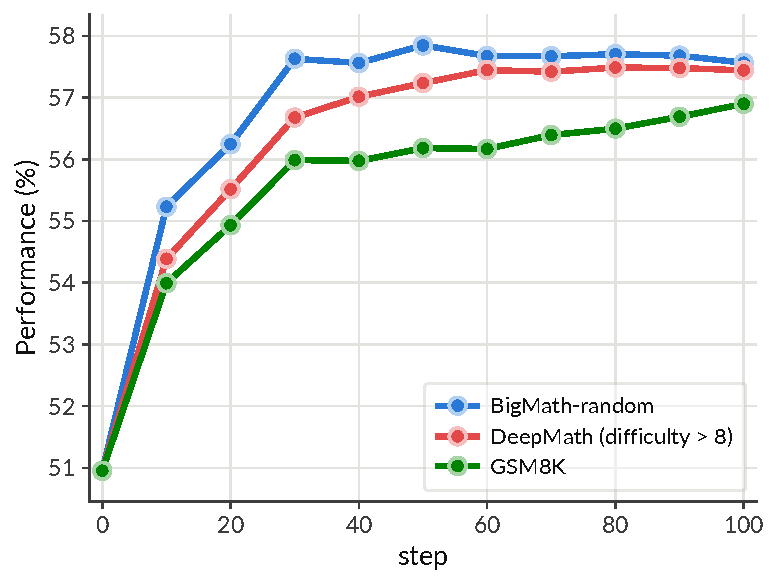
\includegraphics[width=\linewidth]{latex/figures/findings_1/teacher_pass_rate/7b_to_7b_math_teacher_difficulty_mainmath6_avg.pdf}
        \caption{Polaris-7B $\rightarrow$ DS-distill-7B}
        \label{fig:difficulty_7b_to_7b}
    \end{subfigure}

    \caption{领域内数学性能（六个英文基准的平均值）对训练查询的难度变化不敏感。子图（a--c）分别在极简单的GSM8K、极困难的DeepMath-103K以及多样化的BigMath混合数据集上进行训练。}
    \label{fig:extreme_difficulty}
\end{figure*}

\subsection{模型原点的额外泛化结果}
\label{sec:appendix_additional_generalization}


图~\ref{fig:math_generalization_and_code_generalization} 展示了在三种教师-学生配置下的额外泛化结果。每个面板报告了在英文数学、中文数学、长时序数学和代码任务上的性能，使我们能够共同考察领域内分布变化和跨领域迁移。

图~\ref{fig:4b_to_4b} 展示了同源的 Polaris-4B $\rightarrow$ Qwen3-4B 配置。  
我们对比了在随机采样的 Big-Math-RL-Verified 子集上的 OPD 与在 Polaris-53K（Polaris-4B 后训练所用数据集）上的 OPD。  
两种训练分布均产生稳定的性能提升，并在评估基准上收敛至相似水平。  
该结果表明，有效的 OPD 并不需要访问教师模型原始的后训练数据。  
图~\ref{fig:32b_to_8b} 报告了跨源的 Qwen3-32B $\rightarrow$ Qwen3-8B-SFT 配置，其在 Big-Math-RL-Verified 上进行训练。  
Qwen3-8B-SFT 从 Qwen3-8B-Base 初始化，并在 OPD 前基于 OpenThoughts3-1.2M 进行监督微调。  
学生模型在英文数学、中文数学以及长时序数学任务上均有明显提升，表明数学监督能够有效跨越语言和推理时序的变化实现迁移。  
相比之下，代码性能仅发生微小变化。  
该结果说明，在跨源师生配置下，广泛领域的泛化能力并不必然意味着对每个语义领域都具有同等强度的迁移效果。  
图~\ref{fig:14b_to_14b} 展示了同源的 Light-R1-14B $\rightarrow$ DS-distill-14B 配置。  
OPD 在所有四个评估组中均带来稳定提升。  
尤为值得注意的是，在长时序数学任务上，蒸馏后的学生模型最终以显著优势超越独立教师模型。  
这一观察表明，最终的学生模型并不必然受限于教师模型独立基准下的准确率。

\subsection{完整的跨领域迁移结果}
\label{sec:appendix_complete_others_to_math}

图~\ref{fig:cross_domain_generalization_others_to_math} 展示了从代码和科学训练数据迁移到数学推理的完整结果。第一行展示了 DS-distill-1.5B 的结果，第二行则展示了 DS-distill-7B 的对应结果。对于每个学生模型，我们评估了英文数学、中文数学以及长时序数学问题的表现。在两种模型大小下，使用代码或科学查询的 OPD 通常能提升数学推理能力，尽管这些实验中并未使用任何数学查询。这种提升不仅体现在标准英文基准上，还扩展到了中文问题和组合型长时序问题。这证实了教师的数学能力可以通过从非数学领域收集的学生轨迹实现迁移。

完整的曲线进一步证实了主文中报告的模型-原点效应。同源教师在三个评估分布上通常产生更强且更稳定的提升。在同一教师谱系内，数学、代码和科学监督实验之间的差异相对较小，而改变教师原点则会产生更大的性能差距。因此，教师-学生后训练关系对跨领域迁移的影响，可能比训练查询的名义领域更具影响力。

我们进一步考察了指令遵循数据是否可以作为数学能力迁移的载体。图~\ref{fig:if_to_math_cross_domain_generalization} 报告了 Nemotron-1.5B $\rightarrow$ DS-distill-1.5B 以及 Polaris-7B $\rightarrow$ DS-distill-7B 的结果。两种配置均在英文数学、中文数学上进行了评估。即使学生轨迹是从指令遵循提示中收集的，教师仍然能够传递那些未在名义训练领域中明确表示的能力。结合之前的结果，这表明训练查询主要决定了教师监督的触发位置，而非严格限制哪些教师能力可以被迁移。

\subsection{MOPD 的完整数学结果}
\label{sec:appendix_mopd_full_math}

表~\ref{tab:mopd_math_full_result} 报告了 MOPD 实验在训练步数 200 时的完整数学推理结果。  
在第一种教师–领域分配方案下，JustRL 提供数学监督，Nemotron 提供科学/IF 监督。  
以 JustRL 为主导的混合方案通常保持更强的数学性能。  
$25/8$ 配置实现了最高的平均得分 $19.6\%$，略高于仅使用 JustRL 的配置以及均衡的 $1/1$ 混合方案。  
此外，一旦 Nemotron 成为主导，数学性能便显著下降：  
平均得分从均衡混合方案的 $19.1\%$ 下降至 $17.4\%$（对应 $2/25$）以及 Nemotron 单独配置的 $14.9\%$。  
该关系在各个基准上并非严格单调，但总体趋势表明，过多的 Nemotron 监督会使学生偏向 Nemotron 较弱的数学能力。

反向分配提供了互补的证据。在此情景中，Nemotron 监督数学查询，而 JustRL 监督科学/IF 查询。尽管进行了这种重新分配，增加 JustRL 监督的比例仍能提升学生在数学任务上的表现。仅使用 JustRL 的配置平均得分为 $17.5\%$，而平衡配置和仅使用 Nemotron 的配置分别为 $15.8\%$。这一结果无法通过名义上的训练领域分配来解释，因为在该情景下，JustRL 并不监督数学数据。相反，其更强的数学能力是通过科学/IF 轨迹实现迁移的。因此，完整的基准测试结果证实，领域路由并不会将教师的影响限制在其指定的领域内。


\begin{figure*}[t]
    \centering

    \begin{subfigure}[b]{0.99\linewidth}
        \centering
        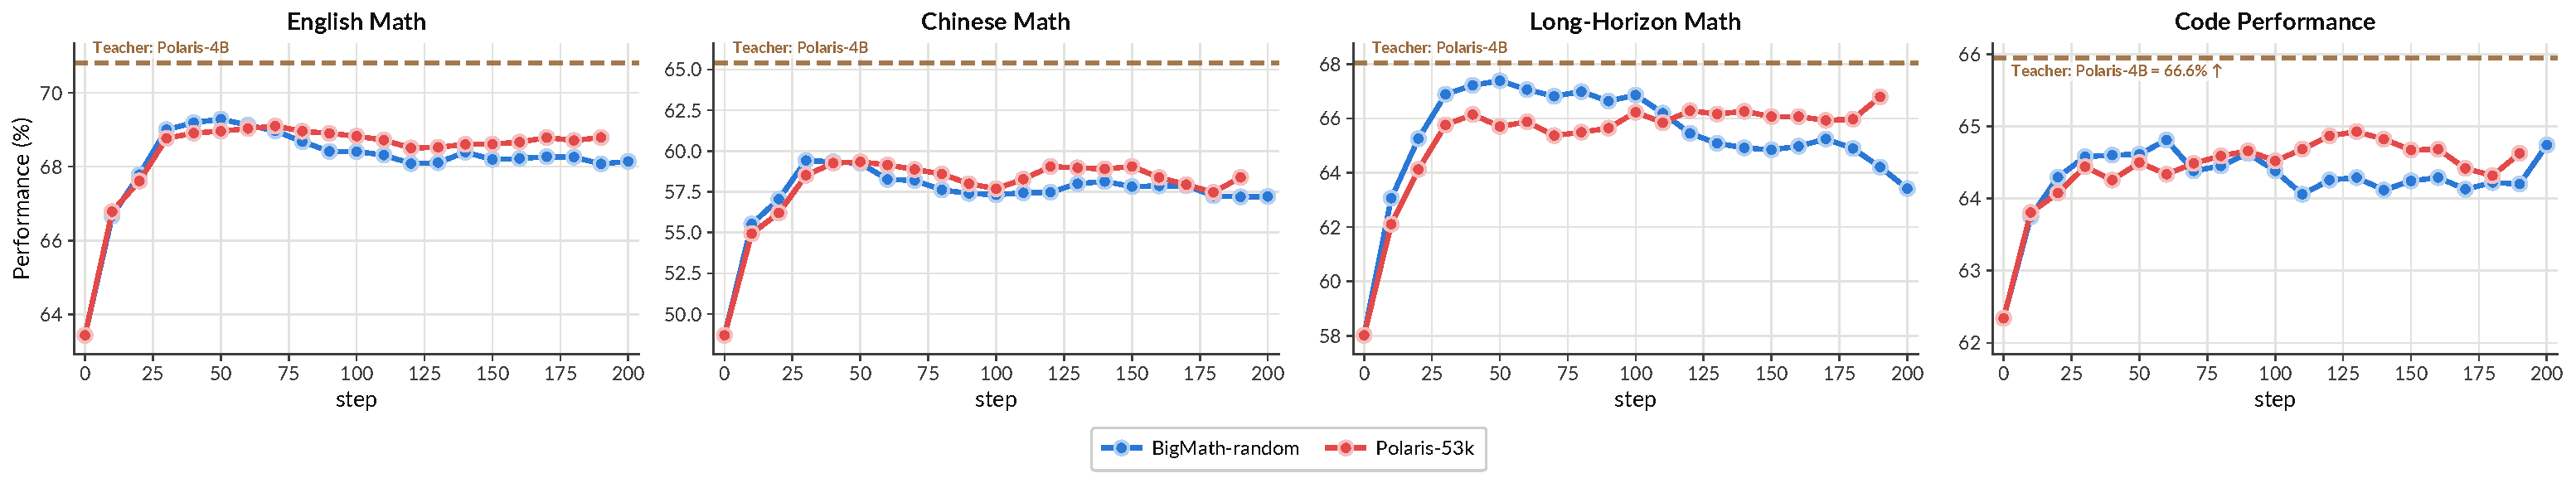
\includegraphics[width=\linewidth]{latex/figures/appendix/4b_polaris4b_qwen3_generalization_math_panel.pdf}
        \caption{Polaris-4B 到 Qwen3-4B}
        \label{fig:4b_to_4b}
    \end{subfigure}

    \begin{subfigure}[b]{0.99\linewidth}
        \centering
        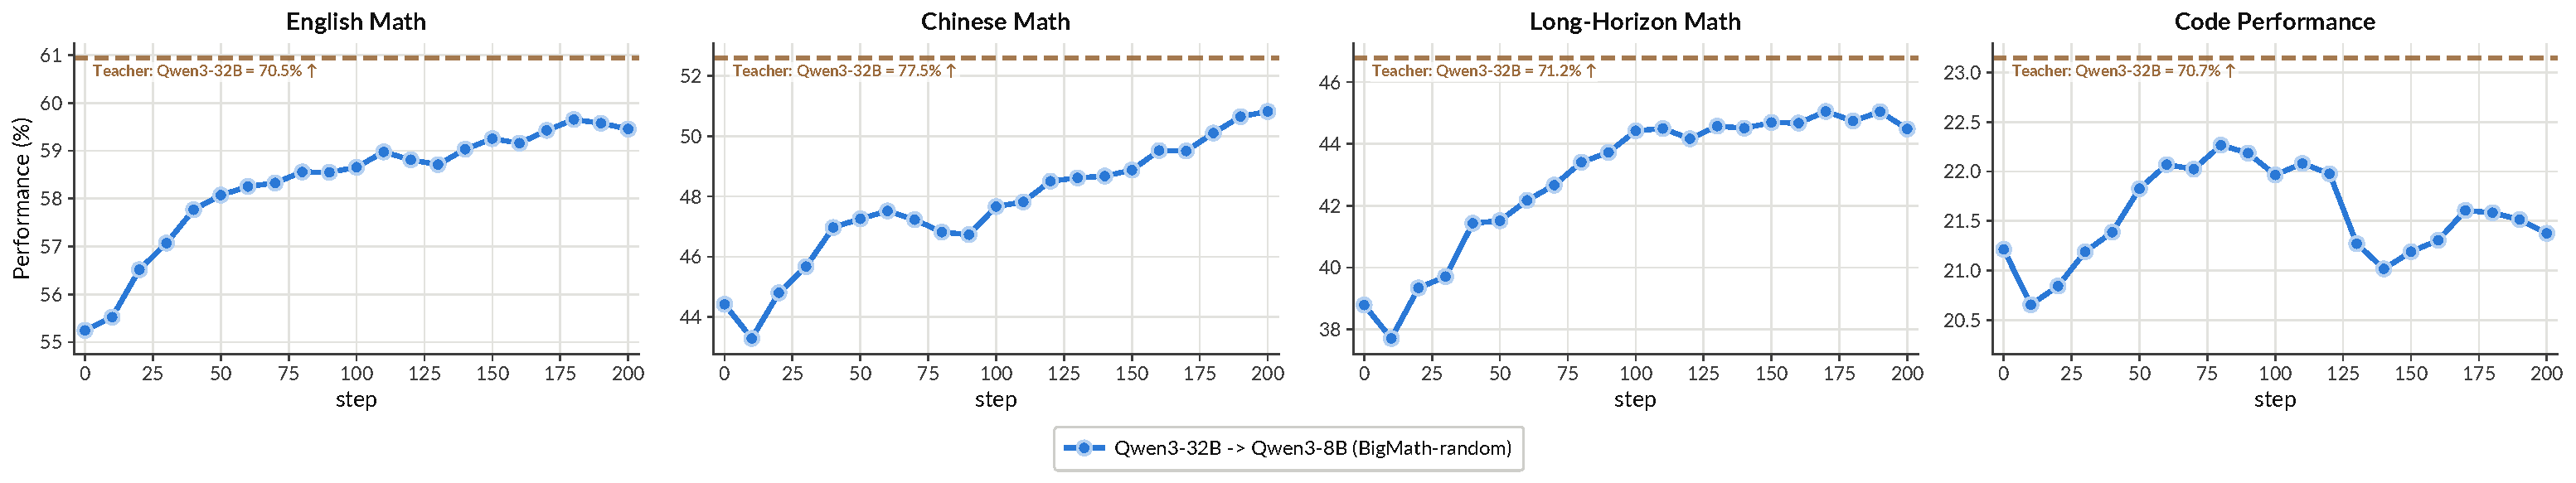
\includegraphics[width=\linewidth]{latex/figures/appendix/8b_qwen32b_bigmath_generalization_math_panel.pdf}
        \caption{Qwen3-32B 到 Qwen3-8B-SFT}
        \label{fig:32b_to_8b}
    \end{subfigure}

     \begin{subfigure}[b]{0.99\linewidth}
        \centering
        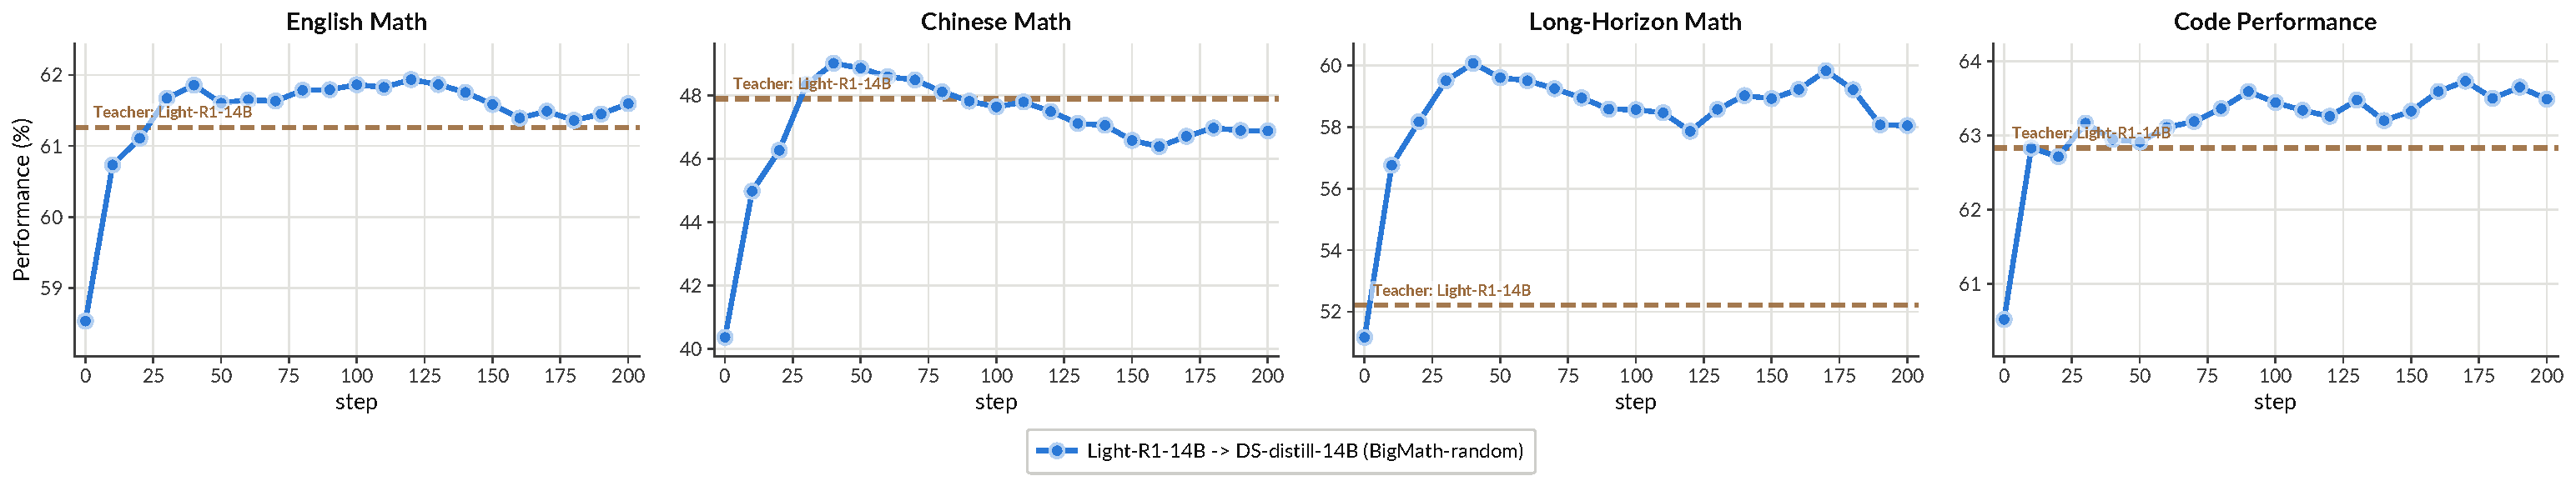
\includegraphics[width=\linewidth]{latex/figures/appendix/14b_lightr1_bigmath_generalization_math_panel.pdf}
        \caption{Light-R1-14B 到 DS-distill-14B}
        \label{fig:14b_to_14b}
    \end{subfigure}

    \caption{在三种教师-学生配置下的额外泛化结果。}
    \label{fig:math_generalization_and_code_generalization}
\end{figure*}

\begin{figure*}[t]
    \centering
    \captionsetup[subfigure]{font=scriptsize}
    \begin{subfigure}[b]{0.32\linewidth}
        \centering
        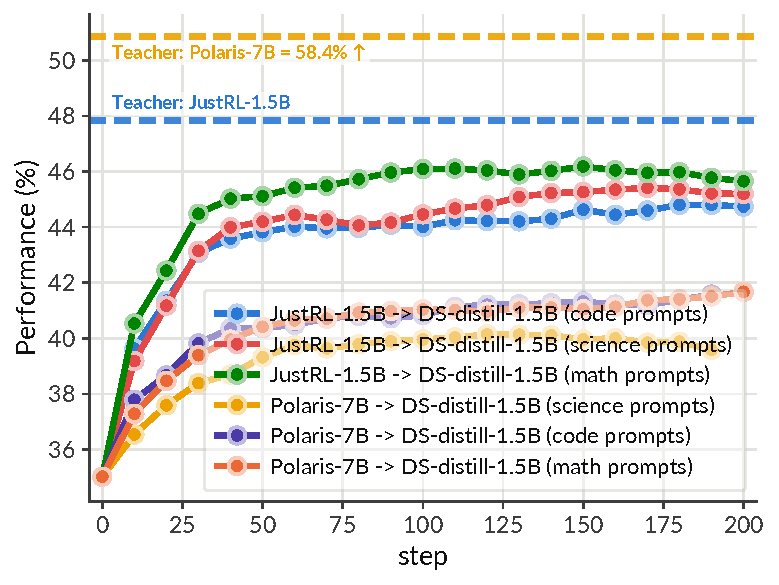
\includegraphics[width=\linewidth]{latex/figures/findings_2/1d5b_cross_domain_generalization_others_to_math_mainmath6_avg.pdf}
        \caption{数学（DS-distill-1.5B）}
        \label{fig:others_to_math_en_1d5b}
    \end{subfigure}
    \hfill
    \begin{subfigure}[b]{0.32\linewidth}
        \centering
        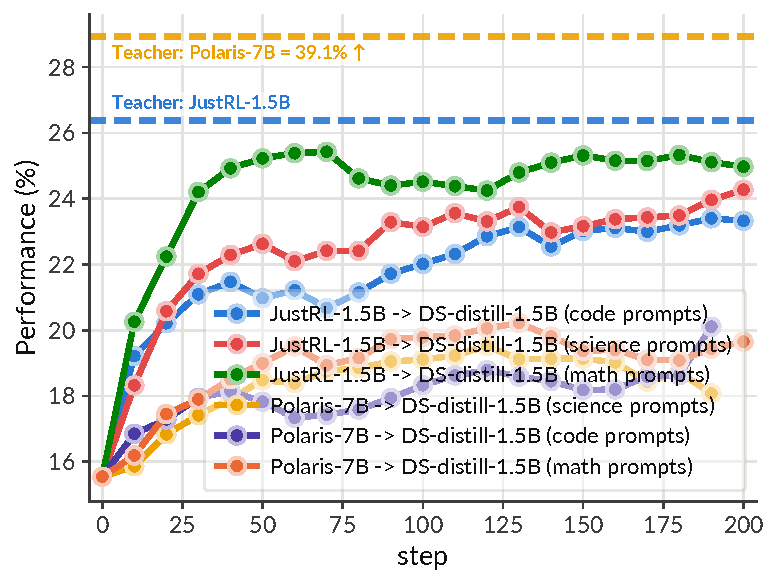
\includegraphics[width=\linewidth]{latex/figures/findings_2/1d5b_cross_domain_generalization_others_to_math_zh_avg.pdf}
        \caption{中国数学（DS-distill-1.5B）}
        \label{fig:others_to_math_zh_1d5b}
    \end{subfigure}
    \hfill
    \begin{subfigure}[b]{0.32\linewidth}
        \centering
        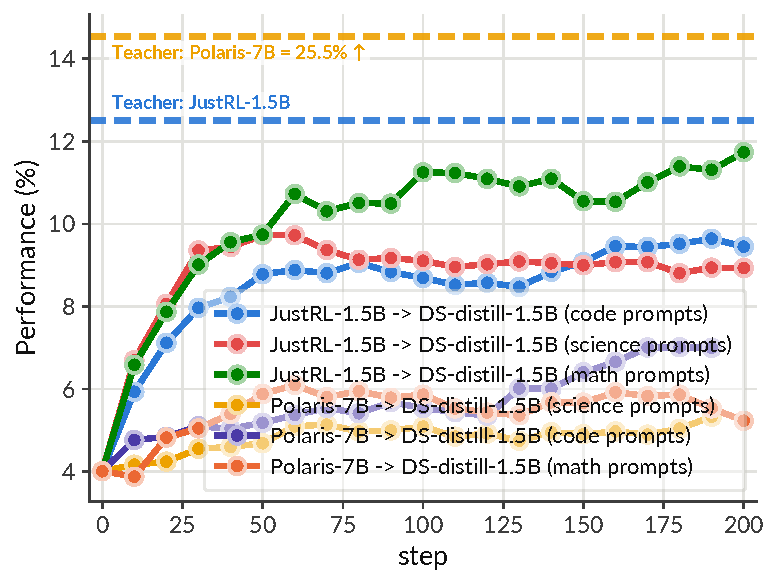
\includegraphics[width=\linewidth]{latex/figures/findings_2/1d5b_cross_domain_generalization_others_to_math_horizon_avg.pdf}
        \caption{长时程数学（DS-distill-1.5B）}
        \label{fig:others_to_math_horizon_1d5b}
    \end{subfigure}

     \begin{subfigure}[b]{0.32\linewidth}
        \centering
        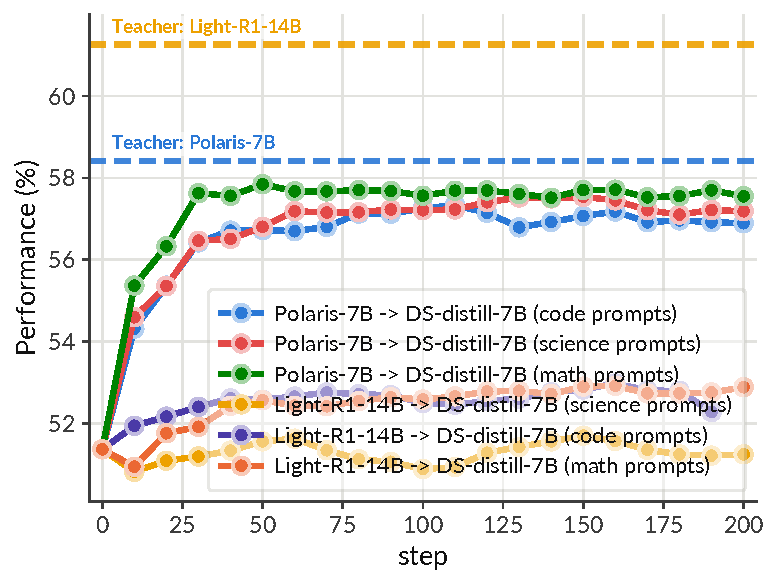
\includegraphics[width=\linewidth]{latex/figures/findings_2/7b_cross_domain_generalization_others_to_math_mainmath6_avg.pdf}
        \caption{数学（DS-distill-7B）}
        \label{fig:others_to_math_en_7b}
    \end{subfigure}
    \hfill
    \begin{subfigure}[b]{0.32\linewidth}
        \centering
        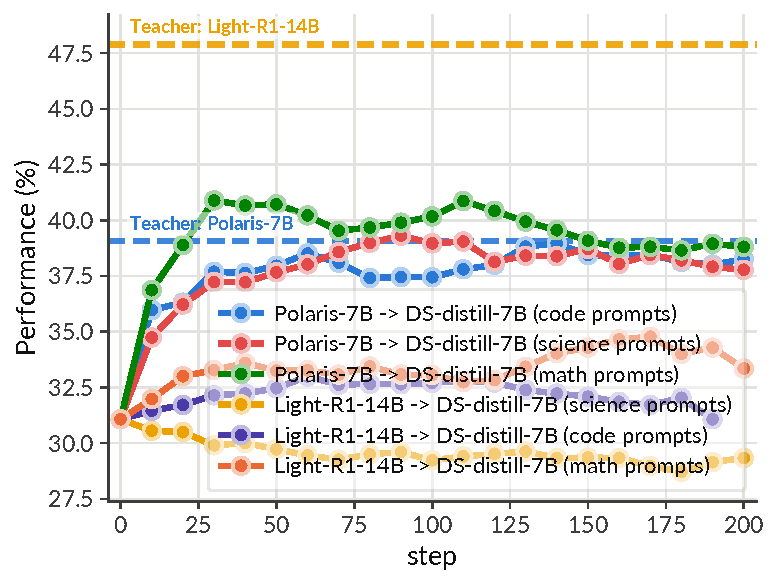
\includegraphics[width=\linewidth]{latex/figures/findings_2/7b_cross_domain_generalization_others_to_math_zh_avg.pdf}
        \caption{中文数学（DS-distill-7B）}
        \label{fig:others_to_math_zh_7b}
    \end{subfigure}
    \hfill
    \begin{subfigure}[b]{0.32\linewidth}
        \centering
        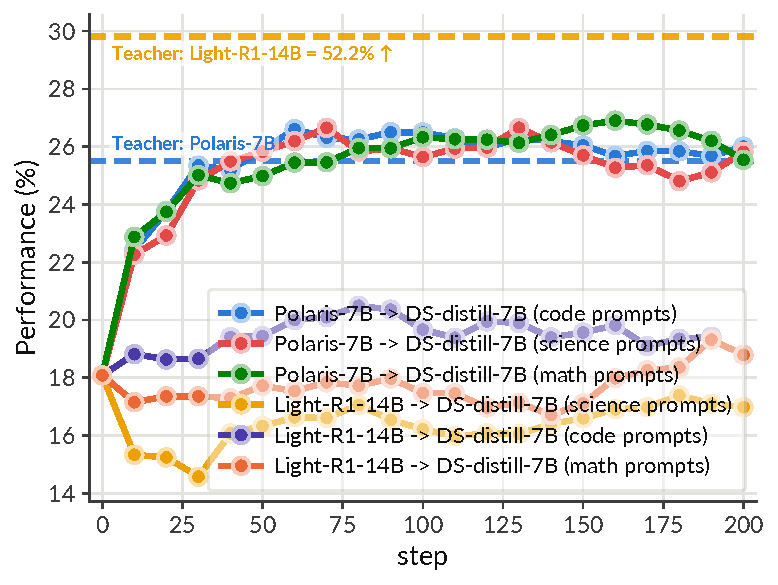
\includegraphics[width=\linewidth]{latex/figures/findings_2/7b_cross_domain_generalization_others_to_math_horizon_avg.pdf}
        \caption{长时程数学（DS-distill-7B）}
        \label{fig:others_to_math_horizon_7b}
    \end{subfigure}

    \caption{在代码和科学领域进行训练，并泛化到与数学相关的领域。}
    \label{fig:cross_domain_generalization_others_to_math}
\end{figure*}


\begin{figure*}[t]
    \centering
    \begin{subfigure}[b]{0.99\linewidth}
        \centering
        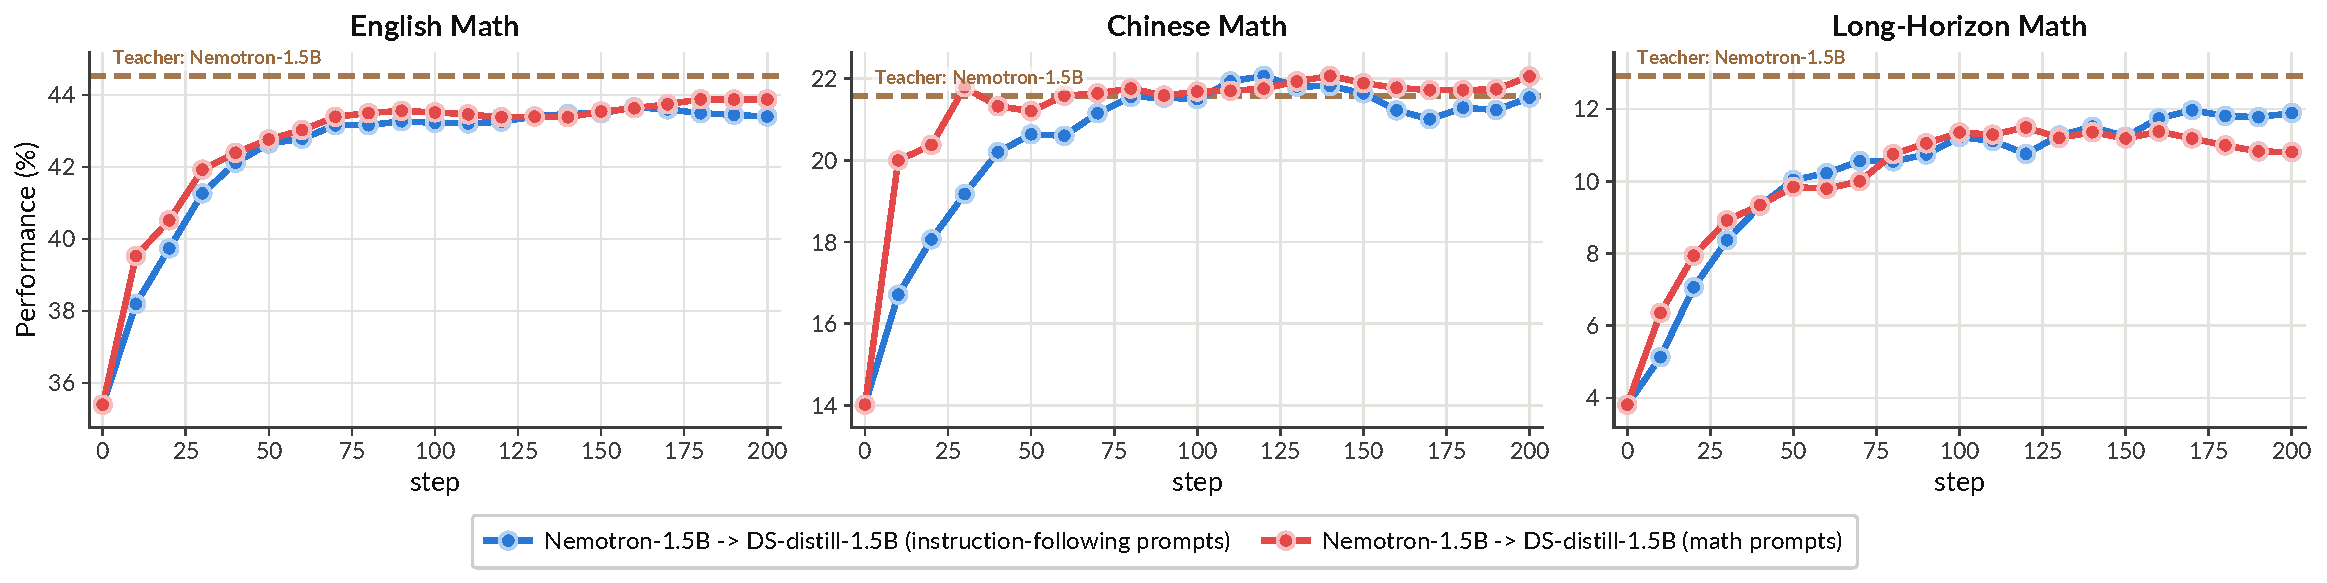
\includegraphics[width=\linewidth]{latex/figures/appendix/1d5b_nemo_if_to_math_generalization_math_panel.pdf}
        \caption{Nemotron-1.5B 到 DS-distill-1.5B}
        \label{fig:if_to_math_1d5b}
    \end{subfigure}

     \begin{subfigure}[b]{0.99\linewidth}
        \centering
        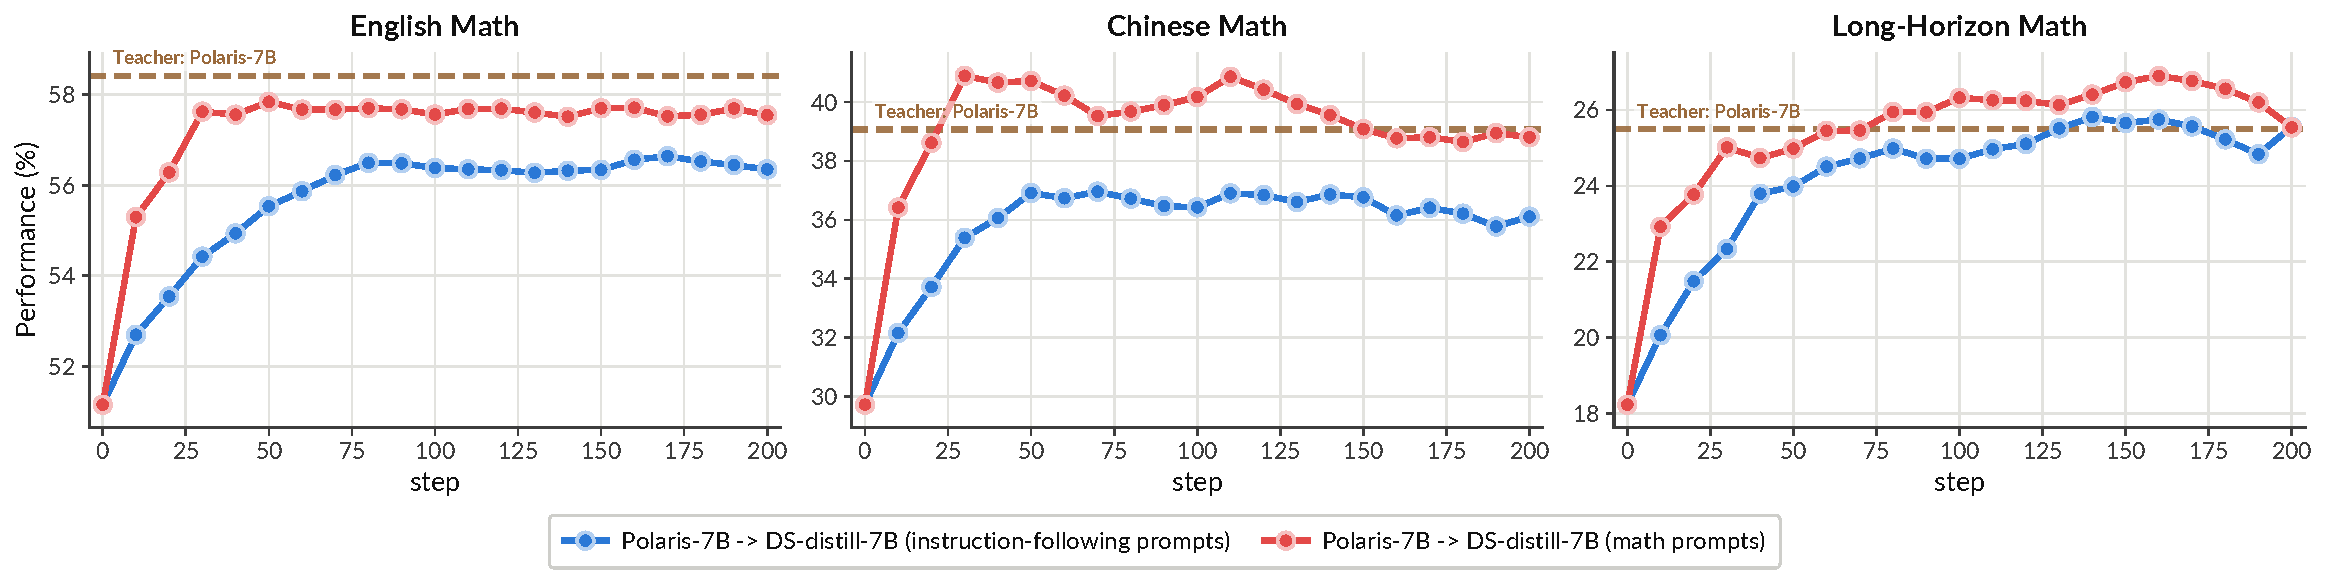
\includegraphics[width=\linewidth]{latex/figures/appendix/7b_polaris_if_to_math_generalization_math_panel.pdf}
        \caption{北斗七B至DS提炼七B}
        \label{fig:if_to_math_7b}
    \end{subfigure}

    \caption{在指令遵循数据上进行训练，并在数学相关基准上实现泛化。}
    \label{fig:if_to_math_cross_domain_generalization}
\end{figure*}

\begin{table*}[htbp]
\centering
\caption{MOPD 在五个数学推理基准上的性能比较（训练步数为200）。}
\label{tab:mopd_math_full_result}
\resizebox{\textwidth}{!}{%
\begin{tabular}{c|ccccc|c}
\toprule
\textbf{Configuration} & \textbf{BeyondAIME} & \textbf{OlymMATH-e(en)} & \textbf{OlymMATH-e(zh)} & \textbf{OlymMATH-h} & \textbf{AIME24-n2} & \textbf{Average} \\
\midrule
\midrule
DS-distill-1.5B & $9.6\%$ & $14.2\%$ & $11.2\%$ & $3.2\%$ & $6.0\%$ & $8.8\%$ \\
JustRL-1.5B & $19.0\%$ & $32.6\%$ & $23.0\%$ & $5.7\%$ & $16.3\%$ & $19.3\%$ \\
Nemotron-1.5B & $17.6\%$ & $29.2\%$ & $16.6\%$ & $5.6\%$ & $14.3\%$ & $16.7\%$ \\
\midrule
\midrule
\multicolumn{7}{c}{\textbf{\textit{Math Teacher: JustRL-1.5B, science/IF Teacher: Nemotron-1.5B, Student: DS-distill-1.5B}}} \\
\midrule

$\mathbf{\text{JustRL}/\text{Nemotron}=25/0}$ & $19.0\%$ & $32.6\%$ & $23.0\%$ & $5.7\%$ & $16.3\%$ & $19.3\%${\footnotesize \textcolor{green!60!black}{(\textbf{+0.2 pp})}} \\
$\mathbf{\text{JustRL}/\text{Nemotron}=25/2}$ & $19.4\%$ & $33.3\%$ & $23.0\%$ & $5.9\%$ & $14.1\%$ & $19.1\%${\footnotesize \textcolor{gray!60!black}{(\textbf{+0.0 pp})}} \\
$\mathbf{\text{JustRL}/\text{Nemotron}=25/8}$ & $19.6\%$ & $34.5\%$ & $23.2\%$ & $5.5\%$ & $15.3\%$ & $19.6\%${\footnotesize \textcolor{green!60!black}{(\textbf{+0.5 pp})}} \\
$\mathbf{\text{JustRL}/\text{Nemotron}=1/1}$ & $20.2\%$ & $32.4\%$ & $20.6\%$ & $5.0\%$ & $17.3\%$ & $19.1\%${\footnotesize \textcolor{black!60!black}{(\textbf{baseline})}} \\
$\mathbf{\text{JustRL}/\text{Nemotron}=8/25}$ & $19.7\%$ & $32.5\%$ & $22.7\%$ & $5.5\%$ & $15.7\%$ & $19.2\%${\footnotesize \textcolor{green!60!black}{(\textbf{+0.1 pp})}} \\
$\mathbf{\text{JustRL}/\text{Nemotron}=2/25}$ & $19.2\%$ & $31.0\%$ & $19.2\%$ & $5.2\%$ & $12.3\%$ & $17.4\%${\footnotesize \textcolor{red!60!black}{(\textbf{-1.7 pp})}} \\
$\mathbf{\text{JustRL}/\text{Nemotron}=0/25}$ & $15.9\%$ & $25.3\%$ & $15.7\%$ & $3.7\%$ & $13.8\%$ & $14.9\%${\footnotesize \textcolor{red!60!black}{(\textbf{-4.2 pp})}} \\

\midrule
\midrule
\multicolumn{7}{c}{\textbf{\textit{Math Teacher: Nemotron-1.5B, science/IF Teacher: JustRL-1.5B, Student: DS-distill-1.5B}}} \\
\midrule

$\mathbf{\text{JustRL}/\text{Nemotron}=25/0}$ & $18.2\%$ & $29.8\%$ & $21.1\%$ & $5.8\%$ & $12.3\%$ & $17.5\%${\footnotesize \textcolor{green!60!black}{(\textbf{+1.7 pp})}} \\
$\mathbf{\text{JustRL}/\text{Nemotron}=25/8}$ & $17.4\%$ & $28.0\%$ & $17.8\%$ & $4.5\%$ & $14.8\%$ & $16.5\%${\footnotesize \textcolor{green!60!black}{(\textbf{+0.7 pp})}} \\
$\mathbf{\text{JustRL}/\text{Nemotron}=1/1}$ & $17.3\%$ & $26.6\%$ & $16.8\%$ & $4.4\%$ & $13.9\%$ & $15.8\%${\footnotesize \textcolor{black!60!black}{(\textbf{baseline})}} \\
$\mathbf{\text{JustRL}/\text{Nemotron}=8/25}$  & $17.1\%$ & $26.2\%$ & $16.8\%$ & $4.7\%$ & $14.3\%$ & $15.8\%${\footnotesize \textcolor{gray!60!black}{(\textbf{-0.0 pp})}} \\
$\mathbf{\text{JustRL}/\text{Nemotron}=0/25}$ & $17.4\%$ & $26.5\%$ & $17.0\%$ & $4.5\%$ & $13.6\%$ & $15.8\%${\footnotesize \textcolor{gray!60!black}{(\textbf{-0.0 pp})}} \\
\bottomrule
\end{tabular}%
}
\end{table*}





\end{document}
